
\documentclass[11pt,french,english,twoside]{book}

%
% macrosHyperlink TeX configuration file
%
% (c) by Olivier Pantalé 2020
%
\usepackage{kurier} % Set the default font for the document
%\usepackage{bookman}
\usepackage{helvet}
\usepackage[T1]{fontenc}
\usepackage[utf8]{inputenc}
\usepackage[a4paper]{geometry}
\geometry{verbose,tmargin=3cm,bmargin=2cm,lmargin=2cm,rmargin=1.5cm,headheight=1cm,headsep=1cm,footskip=1cm}
\pagestyle{headings}
\setcounter{secnumdepth}{4}
\setcounter{tocdepth}{4}
\setlength{\parskip}{\medskipamount}
\setlength{\parindent}{0pt}
\usepackage{color}
\usepackage{array}
\usepackage{babel}
\usepackage{longtable}
\usepackage{multirow}
\usepackage{float}
\usepackage{textcomp}
\usepackage{amsmath}
\usepackage{amssymb}
\usepackage{cancel}
\usepackage{stmaryrd}
\usepackage{graphicx}
\PassOptionsToPackage{normalem}{ulem}
\usepackage{ulem}
\usepackage{float}
\usepackage{cite}
\usepackage{geometry}
\usepackage{lettrine} 
\usepackage{pict2e}
\usepackage{minitoc}
\usepackage{comment}
\usepackage{tikz}
\usepackage{titletoc}
\usepackage{calc}
\usepackage{makeidx}
\usepackage[]{titlesec} 
\usepackage{placeins}
\usepackage{tcolorbox}
\usepackage{tabularx}
\usepackage{array}
\usepackage{colortbl}
\usepackage{fancyhdr}
\usepackage{tablefootnote}
\usepackage[nice]{nicefrac}
\usetikzlibrary{shadows.blur}
\tcbuselibrary{skins}

% Define the macros for color tables
\newcolumntype{L}{>{\raggedleft\arraybackslash}X}
\newcolumntype{R}{>{\raggedright\arraybackslash}X}
\newcolumntype{C}{>{\centering\arraybackslash}X}
\tcbset{myTab/.style={enhanced,fonttitle=\bfseries,fontupper=\normalsize,
colback=gray!10!white,colframe=gray!85!black,colbacktitle=gray,
coltitle=white,center title}}

% Sets the caption of all figures
\usepackage{caption}
\captionsetup[figure]{labelfont={bf,it}, textfont=it}
\captionsetup[table]{labelfont={bf,it}, textfont=it}

% Change the list spaces
\usepackage{enumitem}
\setlist[description]{itemsep=0.3em, parsep=0em, itemindent=-1em}

\makeatletter

% Titre de l'ouvrage
\newcommand{\MyTitle}{Academic year 2020/2021}

%Command for bilingual texts
\newcommand{\frEn}[2]{#2} % Default English

% pour les doubles versions des documents
\newenvironment{fullVersion}{}{}

% Dimensions de la page
\geometry{verbose,a4paper,tmargin=3cm,bmargin=2.5cm,lmargin=2cm,rmargin=2cm,headheight=1cm,headsep=1cm,footskip=1cm}

\pagestyle{fancyplain}
\renewcommand{\floatpagefraction}{1.0}
\renewcommand{\textfraction}{0.2}
\renewcommand{\bottomfraction}{1.0}
\setcounter{tocdepth}{2}
\setcounter{secnumdepth}{3}

% Lettrine
\newcommand{\LETTRINE}[1]{\lettrine[lines=3]{\textcolor{myRed}{#1}}{}}

% style spcial pour les footnotes
\renewcommand\@makefnmark{\@textsuperscript{\normalfont(\@thefnmark)}}

% style special pour les rfrences personnelles
\newcommand{\myCite}[1]{\textbf{\underbar{\cite{#1}~}}}

% modification de la bibliographie
\renewenvironment{thebibliography}[1]
     {\section*{\bibname}%
      \@mkboth{\MakeUppercase\bibname}{\MakeUppercase\bibname}%
      \list{\@biblabel{\@arabic\c@enumiv}}%
           {\settowidth\labelwidth{\@biblabel{#1}}%
            \leftmargin\labelwidth
            \advance\leftmargin\labelsep
            \@openbib@code
            \usecounter{enumiv}%
            \let\p@enumiv\@empty
            \renewcommand\theenumiv{\@arabic\c@enumiv}}%
      \sloppy
      \clubpenalty4000
      \@clubpenalty \clubpenalty
      \widowpenalty4000%
      \sfcode`\.\@m}
     {\def\@noitemerr
       {\@latex@warning{Empty `thebibliography' environment}}%
      \endlist}

\renewcommand{\chaptermark}[1]{\markboth{#1}{}}
\lhead [\fancyplain {\bfseries\thepage} {\bfseries\thepage \\ \textcolor{myGray}{\rule{\textwidth}{2mm}}}]
       {\fancyplain {} {\bfseries\leftmark \\ \textcolor{myGray}{\rule{\textwidth}{2mm}}}}
\rhead [\fancyplain {} {\bfseries\leftmark \\ \textcolor{myGray}{\rule{\textwidth}{2mm}}}]
       {\fancyplain {\bfseries\thepage} {\bfseries\thepage \\ \textcolor{myGray}{\rule{\textwidth}{2mm}}}}
\chead{}
\cfoot{}
\lfoot [{\textcolor{myGray}{\rule{\textwidth}{2mm}}\\ \mbox{\scriptsize{\MyTitle}}}]
       {\textcolor{myGray}{\rule{\textwidth}{2mm}}\\ \mbox{\scriptsize{Olivier PANTALE}}}
\rfoot [{\textcolor{myGray}{\rule{\textwidth}{2mm}}\\ \mbox{\scriptsize{Olivier PANTALE}}}]
       {\textcolor{myGray}{\rule{\textwidth}{2mm}}\\ \mbox{\scriptsize{\MyTitle}}}
\renewcommand{\headrulewidth}{0pt}
\renewcommand{\footrulewidth}{0pt}

% cette ligne est necessaire si il n'y a pas d'algorithme dans le fichier lyx
\@ifundefined{algorithm}{

\newfloat{algorithm}{htbp}{loa}
}

% dfinitions pour les sections en couleur dans le texte
\renewcommand\section{\@startsection {section}{1}{\z@}%
                                   {-3.5ex \@plus -1ex \@minus -.2ex}%
                                   {2.3ex \@plus.2ex}%
                                   {\normalfont\LARGE\bfseries\color{myRed}}}
\renewcommand\subsection{\@startsection{subsection}{2}{\z@}%
                                     {-3.25ex\@plus -1ex \@minus -.2ex}%
                                     {1.5ex \@plus .2ex}%
                                     {\normalfont\Large\bfseries\color{myRed}}}
\renewcommand\subsubsection{\@startsection{subsubsection}{3}{\z@}%
                                     {-3.25ex\@plus -1ex \@minus -.2ex}%
                                     {1.5ex \@plus .2ex}%
                                     {\normalfont\large\bfseries\color{myRed}}}

% le super format pour les chapitres
\colorlet{chpnumbercolor}{black}
%\makeatletter
\let\oldl@chapter\l@chapter
\def\l@chapter#1#2{\oldl@chapter{#1}{\textcolor{chpnumbercolor}{#2}}}

\let\old@dottedcontentsline\@dottedtocline
\def\@dottedtocline#1#2#3#4#5{%
\old@dottedcontentsline{#1}{#2}{#3}{#4}{{\textcolor{chpnumbercolor}{#5}}}}
\makeatother

\titleformat{\chapter}[display]
  {\normalfont\color{myRed}}
  {\filleft\Huge\sffamily\bfseries\chaptertitlename\hspace*{2mm}%
  \begin{tikzpicture}[baseline={([yshift=-.6ex]current bounding box.center)}]
    \node[fill=myRed, circle, text=white] {\thechapter};
  \end{tikzpicture}}
  {1ex}
  {\titlerule[5pt]\vspace*{2ex}\huge\sffamily\itshape}
  []

\titleformat{name=\chapter, numberless}[display]
  {\normalfont\color{myRed}}
  {}
  {1ex}
  {\vspace*{2ex}\huge\sffamily\itshape}
  []

% Command to print the actual minitoc
\newcommand{\printmyminitoc}[1][2]{%
    \vspace*{-5ex}
%    \noindent\hspace*{-0.5\hoffset}\hspace*{-0.5in}\hspace*{-0.5\oddsidemargin}%
    \colorlet{chpnumbercolor}{myRed}%
    \begin{tikzpicture}
    \node[rounded corners, align=left, fill=myGray80, inner sep=5mm]{%
        \color{myRed}%
        \begin{minipage}{0.95\columnwidth}%minipage trick
        \printcontents[chapters]{}{1}{\setcounter{tocdepth}{#1}}
        \end{minipage}};
    \end{tikzpicture}
    \vspace*{5ex}}

\def\@part[#1]#2{%
    \ifnum \c@secnumdepth >-2\relax
      \refstepcounter{part}%
      \addcontentsline{toc}{part}{\thepart\hspace{1em}#1}%
    \else
      \addcontentsline{toc}{part}{#1}%
    \fi
    \markboth{}{}%
    {\centering
     \interlinepenalty \@M
    \textcolor{myRed}{\rule{0.5\textwidth}{4mm}}%  <--- the rule
    \nobreak
    \vskip 5\p@
    \normalfont
     \ifnum \c@secnumdepth >-2\relax
       \huge\bfseries \color{myRed}\partname~\thepart
       \par
       \vskip 20\p@
     \fi
     \Huge \bfseries #2\par}%
    \vskip 5\p@
    \textcolor{myRed}{\rule{\textwidth}{4mm}}%  <--- the rule
    \nobreak
    \vskip 10\p@
    \@endpart}

\def\@endpart{\vfil\newpage
	\setcounter{chapter}{0} %reset the counter between chapters
              \if@twoside
               \if@openright
                \null
                \thispagestyle{empty}%
                \newpage
               \fi
              \fi
              \if@tempswa
                \twocolumn
              \fi}

% creation des programmes
\floatstyle{ruled}
\newfloat{Program}{thp}{lop}[chapter]

% plus de place dans les listes
\renewcommand*\l@figure{\@dottedtocline{1}{1.5em}{3.3em}}
\renewcommand*\l@table{\@dottedtocline{1}{1.5em}{3.3em}}
\renewcommand\listof[2]{%
  \@ifundefined{ext@#1}{\float@error{#1}}{%
    \@ifundefined{chapter}{\def\@tempa{\section*}}%
      {\def\@tempa{\chapter*}}%
    \@tempa{#2\@mkboth{\uppercase{#2}}{\uppercase{#2}}}%
    \@namedef{l@#1}{\@dottedtocline{1}{1.5em}{3.3em}}%
    \@starttoc{\@nameuse{ext@#1}}}}

\AtBeginDocument{
\addto\captionsfrench{
\renewcommand{\figurename}{Figure }
\renewcommand{\tablename}{Tableau }
}}

% les numros incluent le numro de la partie
\renewcommand \thefigure
     {\ifnum \c@part>\z@ \thepart.\fi \ifnum \c@chapter>\z@ \thechapter.\fi \@arabic\c@figure}
\renewcommand \thetable
     {\ifnum \c@part>\z@ \thepart.\fi \ifnum \c@chapter>\z@ \thechapter.\fi \@arabic\c@table}

%Definition des mises en page
\newcommand{\listingfontsscale}{\footnotesize}
\usepackage{esvect}
\usepackage{keystroke}
\usepackage{xstring}
\usepackage{transparent}
\usepackage{xspace}
\usepackage{color}
\usepackage{pdfpages}

% Define the set of colors
\definecolor{myGray}{gray}{0.75}
\definecolor{myGray90}{gray}{0.90}
\definecolor{myGray80}{gray}{0.80}
\definecolor{myGray50}{gray}{0.50}
\definecolor{myGray40}{gray}{0.40}
\definecolor{myRed}{rgb}{0.34,0.05,0.05}  
\definecolor{myLightRed}{rgb}{0.54,0.05,0.05}  
\definecolor{myDarkRed}{rgb}{0.14,0.05,0.05} 
\definecolor{myBlue}{rgb}{0.05,0.05,0.34}  % Blue color
\definecolor{myGreen}{rgb}{0.05,0.34,0.05}  % Green color

% Command to define two texts depending on the current language
\newcommand{\FrEn}[2]{\IfStrEq*{\languagename}{french}{#1}{#2}}

% Redefine the esvector shape to remove overlapping
\def\traitfill@#1#2#3#4{%
  $\m@th\mkern2mu\relax#4#1\mkern-1.5mu %on met \relbaredd au d\'ebut
   \cleaders\hbox{$#4\mkern-0.3mu#2\mkern-0.3mu$}\hfill %remplit avec relbareda
   \mkern-1.5mu#3$%
}

% affect overrightarrow to vv
\renewcommand{\overrightarrow}{\vv}

% définition des commandes locales
% Definition of the C++ special command
\DeclareRobustCommand{\Cpp}
{\valign{\vfil\hbox{##}\vfil\cr 
   \textsf{C\kern-.1em}\cr
   $\hbox{\fontsize{\ssf@size}{0}\textbf{+\kern-0.05em+}}$\cr}%
}

% Definition des listings avec langage par défaut Python
\usepackage{listings}

\lstnewenvironment{CppListing}[1][]
    {\lstset{language=C++,
	keywordstyle=\color{myRed},
	numberstyle=\footnotesize\color{myGray50},
	numbers=left,
	frame=single,xleftmargin=5.0ex,xrightmargin=1.0ex,
	literate={-} { \textrm{-}}{1},
	%otherkeywords={>>>},
	%morekeywords={as,assert,with,yield},
	commentstyle=\color{myGray40},
	stringstyle=\color{myGreen},
	basicstyle=\listingfontsscale\sffamily\upshape,
	escapeinside={(*}{*)},  
	backgroundcolor=\color{myGray90},
	rulecolor=\color{myGray50},
        #1}%
        \noindent\begin{minipage}{\textwidth}\csname\@lst @SetFirstNumber\endcsname\end{minipage}}
        {\csname\@lst @SaveFirstNumber\endcsname}

\lstnewenvironment{FortranListing}[1][]
    {\lstset{language=[77]Fortran,
	keywordstyle=\color{myRed},
	numberstyle=\footnotesize\color{myGray50},
	numbers=left,
	frame=single,xleftmargin=5.0ex,xrightmargin=1.0ex,
	literate={-} { \textrm{-}}{1},
	%otherkeywords={>>>},
	%morekeywords={as,assert,with,yield},
	commentstyle=\color{myGray50},
	stringstyle=\color{myGreen},
	basicstyle=\listingfontsscale\sffamily\upshape,
	escapeinside={(*}{*)},  
	backgroundcolor=\color{myGray90},
	rulecolor=\color{myGray50},
        #1}%
        \noindent\begin{minipage}{\textwidth}\csname\@lst @SetFirstNumber\endcsname\end{minipage}}
        {\csname\@lst @SaveFirstNumber\endcsname}

\lstnewenvironment{PythonListing}[1][]
    {\lstset{language=Python,
	keywordstyle=\color{myRed},
	numberstyle=\footnotesize\color{myGray50},
	numbers=left,
	frame=single,xleftmargin=5.0ex,xrightmargin=1.0ex,
	%float=h,
	literate={-} { \textrm{-}}{1},
	%otherkeywords={>>>},
	morekeywords={as,assert,with,yield},
	commentstyle=\color{myGray40},
	stringstyle=\color{myGreen},
	basicstyle=\listingfontsscale\sffamily\upshape,
	escapeinside={(*}{*)},  
	backgroundcolor=\color{myGray90},
	rulecolor=\color{myGray50},
        #1}%
        \noindent\begin{minipage}{\textwidth}\csname\@lst @SetFirstNumber\endcsname\end{minipage}}
        {\csname\@lst @SaveFirstNumber\endcsname}

\lstnewenvironment{AbaqusListing}[1][]
    {\lstset{language=Python,
	keywordstyle=\color{myRed},
	numberstyle=\footnotesize\color{myGray50},
	numbers=left,
	frame=single,xleftmargin=5.0ex,xrightmargin=1.0ex,
	literate={-} { \textrm{-}}{1},
	%otherkeywords={>>>},
	morekeywords={as,assert,with,yield},
	commentstyle=\color{myGray40},
	stringstyle=\color{myGreen},
	basicstyle=\listingfontsscale\sffamily\upshape,
	escapeinside={(*}{*)},  
	backgroundcolor=\color{myGray90},
	rulecolor=\color{myGray50},
		#1}%
        \noindent\begin{minipage}{\textwidth}\csname\@lst @SetFirstNumber\endcsname\end{minipage}}
        {\csname\@lst @SaveFirstNumber\endcsname}

\lstnewenvironment{BashListing}[1][]
	{\lstset{language=bash,
		keywordstyle=\color{myRed},
		numberstyle=\footnotesize\color{myGray50},
		numbers=left,
		frame=single,xleftmargin=5.0ex,xrightmargin=1.0ex,
		literate={-} { \textrm{-}}{1},
		%otherkeywords={>>>},
		%morekeywords={as,assert,with,yield},
		commentstyle=\color{myGray40},
		stringstyle=\color{myGreen},
		basicstyle=\sffamily\listingfontsscale\upshape,
		escapeinside={(*}{*)},  
		backgroundcolor=\color{myGray90},
		rulecolor=\color{myGray50},
		#1}%
	\noindent\begin{minipage}{\textwidth}\csname\@lst @SetFirstNumber\endcsname\end{minipage}}
{\csname\@lst @SaveFirstNumber\endcsname}

\lstset{language=Python,
keywordstyle=\color{myRed},
numberstyle=\footnotesize\color{myGray40},
numbers=left,
frame=single,xleftmargin=5.0ex,xrightmargin=1.0ex,
literate={-} { \textrm{-}}{1},
%otherkeywords={>>>},
morekeywords={as,assert,with,yield},
commentstyle=\color{myGray50},
stringstyle=\color{myGreen},
basicstyle=\listingfontsscale\sffamily\upshape,
escapeinside={(*}{*)},  
backgroundcolor=\color{white},
rulecolor=\color{myGray50}}
\newcommand{\pyout}[1]{\color{blue}\textsl{#1}}

\newcommand{\TI}[1]{\mbox{\large\ensuremath{\mathsf{#1}}}}
\newcommand{\TII}[1]{\mbox{\large\ensuremath{\mathbb{#1}}}}
\newcommand{\TiI}[1]{\mbox{\large\ensuremath{\mathcal{#1}}}}

%Domaines d'intégration
\newcommand{\Ve}	{\Omega_{x}^{e}}
\newcommand{\Se}	{\Gamma_{x}^{e}}

%Tenseur des contraintes, déformations, etc...
\newcommand{\Sig}	{\mbox{\large\ensuremath{\boldsymbol{\sigma}}}}
\newcommand{\Eps}	{\mbox{\large\ensuremath{\boldsymbol{\varepsilon}}}}
\newcommand{\Alp}	{\mbox{\large\ensuremath{\boldsymbol{\alpha}}}}
\newcommand{\ro}	{\mbox{\large\ensuremath{\boldsymbol{\rho}}}}
\newcommand{\gam}	{\mbox{\large\ensuremath{\boldsymbol{\gamma}}}}
\newcommand{\Gam}	{\mbox{\large\ensuremath{\boldsymbol{\Gamma}}}}
\newcommand{\om}	{\mbox{\large\ensuremath{\boldsymbol{\omega}}}}
\newcommand{\Om}	{\mbox{\large\ensuremath{\boldsymbol{\Omega}}}}
\newcommand{\Fi}	{\mbox{\Large\ensuremath{\boldsymbol{\phi}}}}
\newcommand{\Dev}	{\mbox{\Large\ensuremath{\mathsf{s}}}}

%Tenseur Identité
\newcommand{\IId}	{\mbox{\large\ensuremath{\mathbb{I}}}}
\newcommand{\Iid}	{\mbox{\Large\ensuremath{\mathcal{I}}}}
\newcommand{\Id}  	{\mbox{\large\ensuremath{\mathsf{1}}}}

% Tenseurs A du second, 3eme et 4eme ordre
\newcommand{\A}  	{\mbox{\large\ensuremath{\mathsf{A}}}}
\newcommand{\IiA}	{\mbox{\large\ensuremath{\mathcal{A}}}}
\newcommand{\IIA}	{\mbox{\large\ensuremath{\mathbb{A}}}}
\newcommand{\ia}	{\mbox{\large\ensuremath{\mathsf{a}}}}

%Tenseurs B du second, 3eme et 4eme ordre
\newcommand{\B}		{\mbox{\large\ensuremath{\mathsf{B}}}}
\newcommand{\IiB}	{\mbox{\large\ensuremath{\mathcal{B}}}}
\newcommand{\IIB}	{\mbox{\large\ensuremath{\mathbb{B}}}}
\newcommand{\ib}	{\mbox{\large\ensuremath{\mathsf{b}}}}

% Tenseurs C du second, 3eme et 4eme ordre
\newcommand{\C}		{\mbox{\large\ensuremath{\mathsf{C}}}}
\newcommand{\IiC}	{\mbox{\large\ensuremath{\mathcal{C}}}}
\newcommand{\IIC}	{\mbox{\large\ensuremath{\mathbb{C}}}}

% Tenseurs D du second, 3eme et 4eme ordre
\newcommand{\D}		{\mbox{\large\ensuremath{\mathsf{D}}}}
\newcommand{\IiD}	{\mbox{\large\ensuremath{\mathcal{D}}}}
\newcommand{\IID}	{\mbox{\large\ensuremath{\mathbb{D}}}}

% Tenseurs E du second, 3eme et 4eme ordre
\newcommand{\E}		{\mbox{\large\ensuremath{\mathsf{E}}}}
\newcommand{\IiE}	{\mbox{\large\ensuremath{\mathcal{E}}}}
\newcommand{\IIE}	{\mbox{\large\ensuremath{\mathbb{E}}}}
\newcommand{\e}		{\mbox{\large\ensuremath{\mathsf{e}}}}

% Tenseurs F du second, 3eme et 4eme ordre
\newcommand{\F}		{\mbox{\large\ensuremath{\mathsf{F}}}}
\newcommand{\IiF}	{\mbox{\large\ensuremath{\mathcal{F}}}}
\newcommand{\IIF}	{\mbox{\large\ensuremath{\mathbb{F}}}}
\newcommand{\f}		{\mbox{\large\ensuremath{\mathsf{f}}}}

% Tenseurs H du second, 3eme et 4eme ordre
\newcommand{\G}		{\mbox{\large\ensuremath{\mathsf{G}}}}
\newcommand{\IiG}	{\mbox{\large\ensuremath{\mathcal{G}}}}
\newcommand{\IIG}	{\mbox{\large\ensuremath{\mathbb{G}}}}
\newcommand{\ig}	{\mbox{\large\ensuremath{\mathsf{g}}}}

% Tenseurs H du second, 3eme et 4eme ordre
\newcommand{\iH}	{\mbox{\large\ensuremath{\mathsf{H}}}}
\newcommand{\IiH}	{\mbox{\large\ensuremath{\mathcal{H}}}}
\newcommand{\IIH}	{\mbox{\large\ensuremath{\mathbb{H}}}}

% Tenseurs J du second, 3eme et 4eme ordre
\newcommand{\J}		{\mbox{\large\ensuremath{\mathsf{J}}}}
\newcommand{\IiJ}	{\mbox{\large\ensuremath{\mathcal{J}}}}
\newcommand{\IIJ}	{\mbox{\large\ensuremath{\mathbb{J}}}}

% Tenseurs K du second, 3eme et 4eme ordre
\newcommand{\K}		{\mbox{\large\ensuremath{\mathsf{K}}}}
\newcommand{\IiK}	{\mbox{\large\ensuremath{\mathcal{K}}}}
\newcommand{\IIK}	{\mbox{\large\ensuremath{\mathbb{K}}}}

% Tenseurs L du second, 3eme et 4eme ordre
\newcommand{\iL}	{\mbox{\large\ensuremath{\mathsf{L}}}}
\newcommand{\IiL}	{\mbox{\large\ensuremath{\mathcal{L}}}}
\newcommand{\IIL}	{\mbox{\large\ensuremath{\mathbb{L}}}}

% Tenseurs M du second, 3eme et 4eme ordre
\newcommand{\M}		{\mbox{\large\ensuremath{\mathsf{M}}}}
\newcommand{\IiM}	{\mbox{\large\ensuremath{\mathcal{M}}}}
\newcommand{\IIM}	{\mbox{\large\ensuremath{\mathbb{M}}}}
\newcommand{\m}		{\mbox{\large\ensuremath{\mathsf{m}}}}

% Tenseurs N du second, 3eme et 4eme ordre
\newcommand{\N}		{\mbox{\large\ensuremath{\mathsf{N}}}}
\newcommand{\IiN}	{\mbox{\large\ensuremath{\mathcal{N}}}}
\newcommand{\IIN}	{\mbox{\large\ensuremath{\mathbb{N}}}}
\newcommand{\n}		{\mbox{\large\ensuremath{\mathsf{n}}}}

% Tenseurs P du second, 3eme et 4eme ordre
\newcommand{\iP}	{\mbox{\large\ensuremath{\mathsf{P}}}}
\newcommand{\IiP}	{\mbox{\large\ensuremath{\mathcal{P}}}}
\newcommand{\IIP}	{\mbox{\large\ensuremath{\mathbb{P}}}}
\newcommand{\p}		{\mbox{\large\ensuremath{\mathsf{p}}}}

% Tenseurs Q du second, 3eme et 4eme ordre
\newcommand{\Q}		{\mbox{\large\ensuremath{\mathsf{Q}}}}
\newcommand{\IiQ}	{\mbox{\large\ensuremath{\mathcal{Q}}}}
\newcommand{\IIQ}	{\mbox{\large\ensuremath{\mathbb{Q}}}}
\newcommand{\q}		{\mbox{\large\ensuremath{\mathsf{q}}}}

% Tenseurs R du second, 3eme et 4eme ordre
\newcommand{\R}		{\mbox{\large\ensuremath{\mathsf{R}}}}
\newcommand{\IiR}	{\mbox{\large\ensuremath{\mathcal{R}}}}
\newcommand{\IIR}	{\mbox{\large\ensuremath{\mathbb{R}}}}
\newcommand{\ir}	{\mbox{\large\ensuremath{\mathsf{r}}}}

% Tenseurs S du second, 3eme et 4eme ordre
\newcommand{\iS}	{\mbox{\large\ensuremath{\mathsf{S}}}}
\newcommand{\IIS}	{\mbox{\large\ensuremath{\mathbb{S}}}}
\newcommand{\IiS}	{\mbox{\Large\ensuremath{\mathcal{S}}}}

% Tenseurs T du second, 3eme et 4eme ordre
\newcommand{\T}		{\mbox{\large\ensuremath{\mathsf{T}}}}
\newcommand{\IiT}	{\mbox{\large\ensuremath{\mathcal{T}}}}
\newcommand{\IIT}	{\mbox{\large\ensuremath{\mathbb{T}}}}
\newcommand{\bt}	{\mbox{\large\ensuremath{\mathsf{t}}}}

% Tenseurs U du second, 3eme et 4eme ordre
\newcommand{\U}		{\mbox{\large\ensuremath{\mathsf{U}}}}
\newcommand{\IiU}	{\mbox{\large\ensuremath{\mathcal{U}}}}
\newcommand{\IIU}	{\mbox{\large\ensuremath{\mathbb{U}}}}
\newcommand{\iu}	{\mbox{\large\ensuremath{\mathsf{u}}}}

% Tenseurs V du second, 3eme et 4eme ordre
\newcommand{\V}		{\mbox{\large\ensuremath{\mathsf{V}}}}
\newcommand{\IiV}	{\mbox{\large\ensuremath{\mathcal{V}}}}
\newcommand{\IIV}	{\mbox{\large\ensuremath{\mathbb{V}}}}
\newcommand{\iv}	{\mbox{\large\ensuremath{\mathsf{v}}}}

% Tenseurs W du second, 3eme et 4eme ordre
\newcommand{\W}		{\mbox{\large\ensuremath{\mathsf{W}}}}
\newcommand{\IiW}	{\mbox{\large\ensuremath{\mathcal{W}}}}
\newcommand{\IIW}	{\mbox{\large\ensuremath{\mathbb{W}}}}
\newcommand{\iw}	{\mbox{\large\ensuremath{\mathsf{w}}}}

% Tenseurs X du second, 3eme et 4eme ordre
\newcommand{\X}		{\mbox{\large\ensuremath{\mathsf{X}}}}
\newcommand{\IiX}	{\mbox{\large\ensuremath{\mathcal{X}}}}
\newcommand{\x}		{\mbox{\large\ensuremath{\mathsf{x}}}}
\newcommand{\IIX}	{\mbox{\large\ensuremath{\mathbb{X}}}}

% Tenseurs Y du second, 3eme et 4eme ordre
\newcommand{\Y}		{\mbox{\large\ensuremath{\mathsf{Y}}}}
\newcommand{\IiY}	{\mbox{\large\ensuremath{\mathcal{Y}}}}
\newcommand{\y}		{\mbox{\large\ensuremath{\mathsf{y}}}}
\newcommand{\IIY}	{\mbox{\large\ensuremath{\mathbb{Y}}}}

% Tenseurs Z du second, 3eme et 4eme ordre
\newcommand{\Z}		{\mbox{\large\ensuremath{\mathsf{Z}}}}
\newcommand{\IiZ}	{\mbox{\large\ensuremath{\mathcal{Z}}}}
\newcommand{\z}		{\mbox{\large\ensuremath{\mathsf{z}}}}
\newcommand{\IIZ}	{\mbox{\large\ensuremath{\mathbb{Z}}}}

%Null tensor
\newcommand{\0}		{\mbox{\large\ensuremath{\mathsf{0}}}}

%Commandes spéciales espacements
\newcommand{\Vs}	{\vspace{1cm}}
\newcommand{\vs}	{\vspace{2mm}}

%Commandes spéciales
\newcommand{\tr}	{\mbox{\ensuremath{\mathsf{\,tr\,}}}}
\newcommand{\dev}	{\mbox{\ensuremath{\mathsf{\,dev\,}}}}
\newcommand{\grad}	{\mbox{\ensuremath{\mathsf{\,grad\,}}}}
\newcommand{\Div}	{\mbox{\ensuremath{\mathsf{\,div\,}}}}
\newcommand{\curl}	{\mbox{\ensuremath{\mathsf{\,curl\,}}}}
\renewcommand{\det}	{\mbox{\ensuremath{\mathsf{\,det\,}}}}

\newcommand{\pluseq}{\mathrel{+}=}
\newcommand{\minuseq}{\mathrel{-}=}
\newcommand{\multeq}{\mathrel{*}=}
\newcommand{\diveq}{\mathrel{/}=}

\DeclareMathAlphabet{\mathbxsl}{\encodingdefault}{\rmdefault}{m}{it}
\newcommand{\invI}[1]	{\mbox{\large\ensuremath{\mathbxsl{I_{\mathsf{#1}}}}}}
\newcommand{\invII}[1]	{\mbox{\large\ensuremath{\mathbxsl{II_{\mathsf{#1}}}}}}
\newcommand{\invIII}[1]	{\mbox{\large\ensuremath{\mathbxsl{III_{\mathsf{#1}}}}}}

\newcommand*{\ie}	{\emph{i.e.}\@\xspace}
\newcommand*{\versus}	{\emph{vs.}\@\xspace}
\newcommand*{\eal}	{et \emph{al.}\@\xspace}
\newcommand*{\eg}	{e.g.,\@\xspace}

% Declaration des colorboxes
\RequirePackage{calc}
\newsavebox{\boitetitre}
\newlength{\tempdim}
\newlength{\largeurboitetitre}
\newlength{\hauteurboitetitre}
\newlength{\largeurtitre}

\newcommand{\espacetitre}{1.5}
\newcommand{\decalagetitreg}{1}
\newcommand{\decalagetitred}{5}

\newcommand{\traitressort}[2][1]{%
  \leaders\hrule height#2\hskip0pt plus #1fill\relax}

\newcommand{\traitpasressort}[2][1]{%
  \leaders\hrule height#2\hskip1.5em\relax}

\newcommand{\fixedtitlebox}[3][-0.3ex]{%
  \begin{lrbox}{\boitetitre}\kern\fboxsep\colorbox{myGray80}{#3}\kern\fboxsep\end{lrbox}%
  \settowidth{\largeurboitetitre}{\usebox{\boitetitre}}%
  \settowidth{\largeurtitre}{#2}%
  \settoheight{\hauteurboitetitre}{\usebox{\boitetitre}}%
  \settodepth{\tempdim}{\usebox{\boitetitre}}%
  \addtolength{\hauteurboitetitre}{\tempdim+2\fboxrule+2\fboxrule+2\fboxsep}%
  \parbox{2\fboxrule}{%
    \rule{2\fboxrule}{\hauteurboitetitre}}%
  \parbox{\largeurboitetitre}{%
    \begin{flushleft}
      \makebox[\largeurboitetitre]{%
        \traitpasressort[\decalagetitreg]{2\fboxrule}%
        \raisebox{#1}[0pt][0pt]{%
          \kern\espacetitre\fboxsep\textbf{#2}\kern\espacetitre\fboxsep}%
        \traitressort[\decalagetitred]{2\fboxrule}}\\[\fboxsep]\nointerlineskip
      \usebox{\boitetitre}\\[\fboxsep]\nointerlineskip%
      \rule{\largeurboitetitre}{2\fboxrule}
    \end{flushleft}}%
  \parbox{\fboxrule}{%
    \rule{2\fboxrule}{\hauteurboitetitre}}}

\newcommand{\titlebox}[3][-0.3ex]{%
  \begin{lrbox}{\boitetitre}\kern\fboxsep\colorbox{myGray80}{#3}\kern\fboxsep\end{lrbox}%
  \settowidth{\largeurboitetitre}{\usebox{\boitetitre}}%
  \settowidth{\largeurtitre}{#2}%
  \settoheight{\hauteurboitetitre}{\usebox{\boitetitre}}%
  \settodepth{\tempdim}{\usebox{\boitetitre}}%
  \addtolength{\hauteurboitetitre}{\tempdim+2\fboxrule+2\fboxrule+2\fboxsep}%
  \parbox{2\fboxrule}{%
    \rule{2\fboxrule}{\hauteurboitetitre}}%
  \parbox{\largeurboitetitre}{%
    \begin{flushleft}
      \makebox[\largeurboitetitre]{%
        \traitressort[\decalagetitreg]{2\fboxrule}%
        \raisebox{#1}[0pt][0pt]{%
          \kern\espacetitre\fboxsep\textbf{#2}\kern\espacetitre\fboxsep}%
        \traitressort[\decalagetitred]{2\fboxrule}}\\[\fboxsep]\nointerlineskip
      \usebox{\boitetitre}\\[\fboxsep]\nointerlineskip%
      \rule{\largeurboitetitre}{2\fboxrule}
    \end{flushleft}}%
  \parbox{\fboxrule}{%
    \rule{2\fboxrule}{\hauteurboitetitre}}}



% Symboles des drives
\renewcommand{\bullet}{\begin{picture}(3,2)\put(1.5,1){\circle*{2}}\end{picture}}

\ifx\pdfoutput\undefined
\usepackage[ps2pdf,pagebackref=true,colorlinks=true,linkcolor=myRed,citecolor=myRed]{hyperref}
\else
\usepackage[pdftex,pagebackref=true,colorlinks=true,linkcolor=myRed,citecolor=myRed]{hyperref}
\fi
\makeindex

\newcommand{\DynELA}{DynELA Finite Element Code}

\excludecomment{fullVersion}

\makeatother


\begin{document}
\includepdf[pages=1-2]{pageGarde.pdf}

\dominitoc\renewcommand{\thepage}{\roman{page}}\setcounter{page}{1}

\tableofcontents{}

\listoffigures

\listoftables

\cleardoublepage

\renewcommand{\thepage}{\arabic{page}}\setcounter{page}{1}

\part{DynELA FEM code theory}

\selectlanguage{french}%

\chapter*{Notations\addcontentsline{toc}{chapter}{Notations}\markboth{Notations}{Notations}}

\frEn
{\LETTRINE{D}'un point de vue général, il est habituel de constater que dans le domaine de la mécanique, comme dans d'autres domaines sûrement, une des principales difficultés vient de la non homogénéité des notations entre les différents auteurs. Il est alors aisé de rendre complètement incompréhensible la moindre théorie lorsque l'on décide de changer de notation. La notion de notation universelle n'étant pas encore d'actualité (même si certaines conventions peuvent être assimilées à des concepts universels), on présente alors ci-dessous le jeu de notations utilisé tout au long de ce document et de manière plus large dans les autres documents faisant partie de cette même série.}
{\LETTRINE{F}rom a general point of view, it is usual to observe that one of the main difficulties in the field of mechanics, as in other fields, is the non-homogeneity of notations between the various authors. It is then easy to make completely incomprehensible the slightest theory when one decides to change notation. As the notion of universal notation is not yet valid (even if certain conventions can be assimilated to universal concepts), then we present below the set of notations used throughout this document and in a broader way in all the other documents in that series.}

\subsection*{\frEn{Conventions de notations}{Notations Conventions}\vspace{-1ex}}

\begin{longtable}[l]{>{\raggedright}p{0.2\paperwidth}>{\raggedright}p{0.8\paperwidth}}
$a$ & \frEn{Scalaire}
{Scalar}\tabularnewline
$\overrightarrow{a}$ & \frEn{Vecteur}
{Vector} \tabularnewline
$\A$ & \frEn{Tenseur d'ordre $2$ ou matrice}
{$2^{nd}$ order Tensor or matrix}\tabularnewline
$\IiA$ & \frEn{Tenseur d'ordre $3$}
{$3^{rd}$ order Tensor}\tabularnewline
$\IIA$ & \frEn{Tenseur d'ordre $4$}
{$4^{th}$ order Tensor}\tabularnewline
\end{longtable}

\subsection*{\frEn{Opérateurs linéaires et mathématiques}{Linear Algebra and Mathematical Operators}\vspace{-1ex}}

\begin{longtable}[l]{>{\raggedright}p{0.2\paperwidth}>{\raggedright}p{0.8\paperwidth}}
$\overrightarrow{a}\cdot\overrightarrow{b}$ & \frEn{Produit scalaire des vecteurs $\overrightarrow{a}$ et $\overrightarrow{b}$}
{Dot product of the vectors $\overrightarrow{a}$ and $\overrightarrow{b}$}\tabularnewline
$\overrightarrow{a}\otimes\overrightarrow{b}$ & \frEn{Produit tensoriel (ou Dyadic) des vecteurs $\overrightarrow{a}$ et $\overrightarrow{b}$}
{Tensor (or Dyadic) product of the vectors $\overrightarrow{a}$ and $\overrightarrow{b}$} \tabularnewline
$\overrightarrow{a}\wedge\overrightarrow{b}$ & \frEn{Produit vectoriel des vecteurs $\overrightarrow{a}$ et $\overrightarrow{b}$}
{Vectorial product of the vectors $\overrightarrow{a}$ and $\overrightarrow{b}$}\tabularnewline
$\A:\B$ & \frEn{Double produit contracté des deux tenseurs $\A$ et $\B$}
{Double contracted product of the two tensors $\A$ et $\B$}\tabularnewline
$\stackrel{\bullet}{\boxempty}$ & \frEn{Dérivée temporelle de la quantité $\boxempty$}
{Time derivative of quantity $\boxempty$}\tabularnewline
$\stackrel{\bullet\bullet}{\boxempty}$ & \frEn{Dérivée seconde temporelle de la quantité $\boxempty$}
{Second order time derivative of quantity $\boxempty$}\tabularnewline
$\boxempty_{,\boxempty}$ & \frEn{Dérivée partielle de la quantité $\boxempty$ par rapport à $_{\boxempty}$}
{Partial derivative of quantity $\boxempty$ with respect to $_{\boxempty}$}\tabularnewline
$\boxempty^{T}$ & \frEn{Transposée d'une matrice ou d'un vecteur $\boxempty$}
{Transpose of a matrix or a vector $\boxempty$}\tabularnewline
$\tr\,\boxempty$ & \frEn{Trace d'une matrice ou d'un tenseur $\boxempty$ ($\tr\,\boxempty=\sum\boxempty_{ii}$)}
{Trace of a matrix or a tensor $\boxempty$ ($\tr\,\boxempty=\sum\boxempty_{ii}$)}\tabularnewline
$\dev\,\boxempty$ & \frEn{Déviateur d'un tenseur $\boxempty$ ($\dev\,\boxempty=\boxempty-\frac{1}{3}\tr\,\boxempty \Id$)}
{Deviatoric part of a tensor $\boxempty$ ($\dev\,\boxempty=\boxempty-\frac{1}{3}\tr\,\boxempty \Id$)}\tabularnewline
$\delta_{ij}$ & \frEn{Identité unitaire de Kronecker}
{Kronecker delta identity}\tabularnewline
$\Id$ & \frEn{Tenseur ou matrice unitaire du deuxième ordre}
{Unity matrix or second order tensor}\tabularnewline
$\IId$ & \frEn{Tenseur unitaire du quatrième ordre}
{Unity fourth order tensor}\tabularnewline
\end{longtable}

\subsection*{\frEn{Mécanique des milieux continus}{Basic Continuum Mechanics}\vspace{-1ex}}

\begin{longtable}[l]{>{\raggedright}p{0.2\paperwidth}>{\raggedright}p{0.8\paperwidth}}
$\overrightarrow{x}=\left[\begin{array}{ccc}
x & y & z\end{array}\right]^{T}$ & \frEn{Coordonnées dans le domaine physique}
{Coordinates in the physical domain}\tabularnewline
$\overrightarrow{u}=\left[\begin{array}{ccc}
u & v & w\end{array}\right]^{T}$ & \frEn{Champ de déplacement}
{Displacement field} \tabularnewline
$\overrightarrow{\omega}=\left[\begin{array}{ccc}
\omega_{x} & \omega_{y} & \omega_{z}\end{array}\right]^{T}$ & \frEn{Champ de rotations}
{Rotation field}\tabularnewline
$\Om$ & \frEn{Volume arbitraire dans la configuration courante}
{Arbitrary body in the current configuration}\tabularnewline
$\Gam$ & \frEn{Frontière d'un volume arbitraire $\Om$ dans la configuration courante}
{Boundary of an arbitrary body $\Om$ in the current configuration}\tabularnewline
$\rho$ & \frEn{Masse volumique du matériau}{}\tabularnewline
$E$ & \frEn{Module de Young d'un matériau}
{Young's modulus of a material}\tabularnewline
$\nu$ & \frEn{Coefficient de Poisson d'un matériau}
{Poisson's ratio of a material}\tabularnewline
$K$ & \frEn{Module de compressibilité d'un matériau}
{Bulk modulus of a material}\tabularnewline
$\lambda$ & \frEn{Premier paramètre de Lamé d'un matériau}
{Lamé's first parameter of a material}\tabularnewline
$\mu=G$ & \frEn{Second paramètre de Lamé / module de cisaillement de Coulomb}
{Lamé's second parameter / Coulomb's shear modulus}\tabularnewline
$\overrightarrow{F}$ & \frEn{Vecteur des efforts externes surfaciques}
{External load vector}\tabularnewline
$\overrightarrow{f}$ & \frEn{Vecteur des efforts externes volumiques}
{External load vector}\tabularnewline
$\Eps$ & \frEn{Tenseur des déformations de Green-Lagrange}
{Green-Lagrange strain tensor}\tabularnewline
$\Sig$ & \frEn{Tenseur des contraintes de Cauchy}
{Cauchy stress tensor}\tabularnewline
$\Dev$ & \frEn{Déviateur du tenseur des contraintes de Cauchy}
{Deviatoric part of the Cauchy stress tensor}\tabularnewline
$\Alp$ & \frEn{Mouvement de l'origine de la surface de charge}
{Backstress tensor}\tabularnewline
$\Fi$ & \frEn{$\Fi=\Dev-\Alp$}
{}\tabularnewline
\end{longtable}

\subsection*{\frEn{Lois de comportement}{Constitutive laws}\vspace{-1ex}}

\begin{longtable}[l]{>{\raggedright}p{0.2\paperwidth}>{\raggedright}p{0.8\paperwidth}}
$f$ & \frEn{Fonction de charge}
{}\tabularnewline
$\n$ & \frEn{Direction de l'écoulement plastique}
{Direction of the plastic flow}\tabularnewline
$\q$ & \frEn{Ensemble des variables d'hérédité dans la formulation élastoplastique}
{Heredity variables in an elastoplastic behavior}\tabularnewline
$\overline{\sigma}$ & \frEn{Contrainte équivalente de von Mises}
{von Mises equivalent stress}\tabularnewline
$\overline{\varepsilon}^{p}$ & \frEn{Déformation plastique équivalente}
{Equivalent plastic strain}\tabularnewline
$\stackrel{\bullet}{\overline{\varepsilon}^{p}}$ & \frEn{Vitesse de déformation plastique équivalente}
{Equivalent plastic strain rate}\tabularnewline
$\Lambda$ & \frEn{Scalaire représentant la norme de l'écoulement plastique}
{Norm of the plastic strain}\tabularnewline
$\sigma^{v}$ & \frEn{Limite apparente d'élasticité du matériau}
{}\tabularnewline
$\sigma_{0}^{v}$ & \frEn{Limite d'élasticité initiale du matériau}
{}\tabularnewline
$\sigma_{\infty}^{v}$ & \frEn{Limite asymptotique de plasticité du matériau}
{}\tabularnewline
\end{longtable}

\subsection*{\frEn{Grandes déformations}{Large Deformations}\vspace{-1ex}}

\begin{longtable}[l]{>{\raggedright}p{0.2\paperwidth}>{\raggedright}p{0.8\paperwidth}}
$\overrightarrow{X}=\left[\begin{array}{ccc}
X & Y & Z\end{array}\right]^{T}$ & \frEn{Coordonnées dans le domaine de référence}
{Coordinates in the reference domain}\tabularnewline
$\E$ & \frEn{Tenseur des déformations de Green-Lagrange}
{Green-Lagrange deformation tensor}\tabularnewline
$\F$ & \frEn{Tenseur gradient de déformation}
{Deformation gradient tensor}\tabularnewline
$\U,\ \V$ & \frEn{Tenseurs des déformations pures droit et gauche}
{Right and left pure deformation tensors}\tabularnewline
$\R$ & \frEn{Tenseur de rotation}
{Rotation tensor}\tabularnewline
$\iL$ & \frEn{Tenseur des vitesses de déformation}
{Deformation speed tensor}\tabularnewline
$\D$ & \frEn{Partie symétrique du tenseur $\iL$}
{Symmetric part of the $\iL$ tensor}\tabularnewline
$\W$ & \frEn{Partie anti-symétrique du tenseur $\iL$}
{Skew-symmetric part of the $\iL$ tensor}\tabularnewline
\end{longtable}

\subsection*{\frEn{Structures de données pour les éléments finis}{Finite Element Data Structures}\vspace{-1ex}}
\begin{flushleft}
\begin{longtable}[l]{>{\raggedright}p{0.2\paperwidth}>{\raggedright}p{0.8\paperwidth}}
$\N$ & \frEn{Matrice des fonctions d'interpolation}
{Shape functions matrix}\tabularnewline
$\overrightarrow{\xi}=\left[\begin{array}{ccc}
\xi & \eta & \zeta\end{array}\right]^{T}$ & \frEn{Coordonnées dans le domaine de parent}
{Coordinates in the parent domain}\tabularnewline
$\B$ & \frEn{Dérivées des fonctions d'interpolation}
{Derivatives of the shape functions}\tabularnewline
$\boxempty^{e}$ & \frEn{Quantité $\boxempty$ relative à l'élément $e$}
{Quantity $\boxempty$ related to element $e$}\tabularnewline
$\J$ & \frEn{Matrice Jacobienne de la transformation physique/parent}
{Jacobian matrix}\tabularnewline
$\M$ & \frEn{Matrice de masse}
{Mass matrix}\tabularnewline
$\K$ & \frEn{Matrice de rigidité}
{Stiffness matrix}\tabularnewline
$\overline{\F}$ & \frEn{Vecteur des efforts externes surfaciques}
{External surfacic load vector}\tabularnewline
$\F$ & \frEn{Vecteur des efforts externes surfaciques et volumiques}
{External load vector}\tabularnewline
$\overline{\f}$ & \frEn{Vecteur des efforts externes volumiques}
{External volumic load vector}\tabularnewline
$\q$ & \frEn{Vecteur des inconnues nodales}
{Nodal unknowns vector}\tabularnewline
$n_{g}$ & \frEn{Nombre de noeuds (généralement) de l'élément}
{Number of nodes of the current element}\tabularnewline
$n_{Q}$ & \frEn{Nombre de points d'intégration de l'élément}
{Number of integration points of the current element}\tabularnewline
\end{longtable}
\par\end{flushleft}\selectlanguage{english}%



\cleardoublepage

\part{DynELA Programming}


\chapter{DynELA programming language}

\startcontents[chapters]
\printmyminitoc[1]\LETTRINE{T}his chapter deals about the \Dynela~programming language.
This language is based on Python 3 and all models must be described
using this formalism. Therefore, this chapter will describe step by
step how to build a Finite Element Model for the \Dynela, using the
Python language.

\section{Introduction}

\subsection{Calling the python interpreter}

After the compilation phase of the code, the \Dynela~can be launch
using the following command:

\textsf{python <'model.py'>}: where model.py is the source Python
3 file defining the \Dynela. The \textsf{model.py }file contains
all the definitions of the Finite Element Model using a Python 3 language
and calling DynELA methods written in \Cpp.

\subsection{Formalism of a DynELA python file}

In order to build a Finite Element Model, it is necessary to import
the \textsf{dnlPython} interpreter from the \textsf{.py} script. Conforming
to this formalism, the minimal piece of Python code to setup a Finite
Element Model is given hereafter.

\begin{PythonListing}
#!/usr/bin/env python3
import dnlPython as dnl # Imports the dnlPython library as dnl
model = dnl.DynELA()    # Creates the main Object
...                     # Set of instructions to build the FE model
                        # and conforming to the DynELA language and Python 3
model.solve()           # Runs the solver
\end{PythonListing}

In the preceding piece of code, line 2 is used to load into memory
the module dnlPython containing the interface to all \Cpp~methods
of the \Dynela~based on the use of the SWIG Python interface. Therefore,
all public methods of the \Dynela~written in \Cpp~can be called
from the Python script to build the FEM model, lanch teh solver, produce
output results... 

In the minimal proposed example, line 3 is used to create an object
of type \textsf{DynELA} (the higher object type in the \Dynela~library)
and instantiate it as the \textsf{model} object\footnote{For the rest of this chapter, we will assume that the name of the
instanciated \textsf{DynELA} object is \textsf{model.}}, while line 6, the solver of the \Dynela~library is called to solve
the problem and produce the results.

As the interpretor of the \Dynela~is based on Python 3 language,
all kind of instructions valid in Python 3 can be used along with
the specific DynELA instructions.

\section{The Kernel library}

\#include \textquotedbl LogFile.h\textquotedbl{}

\#include \textquotedbl MacAddress.h\textquotedbl{}

\#include \textquotedbl Settings.h\textquotedbl{}

\#include \textquotedbl String.h\textquotedbl{}

\#include \textquotedbl System.h\textquotedbl{}

\#include \textquotedbl Timer.h\textquotedbl{}

\#include \textquotedbl Field.h\textquotedbl{}

\section{The Maths library}

\#include \textquotedbl DiscreteFunction.h\textquotedbl{}

\#include \textquotedbl DiscreteFunctionSet.h\textquotedbl{}

\#include \textquotedbl Function.h\textquotedbl{}

\#include \textquotedbl Matrices.h\textquotedbl{}

\#include \textquotedbl Matrix.h\textquotedbl{}

\#include \textquotedbl MatrixDiag.h\textquotedbl{}

\#include \textquotedbl PolynomialFunction.h\textquotedbl{}

\#include \textquotedbl RampFunction.h\textquotedbl{}

\#include \textquotedbl SinusFunction.h\textquotedbl{}

\#include \textquotedbl SymTensor2.h\textquotedbl{}

\#include \textquotedbl Tensor2.h\textquotedbl{}

\#include \textquotedbl Tensor3.h\textquotedbl{}

\#include \textquotedbl Tensor4.h\textquotedbl{}

\#include \textquotedbl Vec3D.h\textquotedbl{}

\#include \textquotedbl Vector.h\textquotedbl{}

\#include \textquotedbl ColorMap.h\textquotedbl{}

\section{Nodes and elements}

All Finite Element Models involves nodes and elements. The very first
part of the model is therefore to create the nodes and the elements
of the structure to setup a FE Model. The \Dynela~library doesn't
include any meshing procedure yet, therefore, it is mandatory to create
all elements and all nodes by hand or using Python loops in case it
can be used. Another way is to use an external meshing program and
convert the output of this program to produce the ad-hoc lines of
Python to describe the elements and the nodes of the model. This has
been used many times by the author, and the Abaqus Finite Element
code, is an efficient way to create the mesh using the .inp text file
generated by the CAE Abaqus program.

\subsection{Definition of the Model}

\subsection{Definition of the nodes}

In the \Dynela, creation of nodes is done by calling the \textsf{DynELA.createNode()}
method. Therefore, a node is created by calling the \textsf{createNode()}
method and giving the new node number and the $x$, $y$ and $z$
coordinates of the new node as presented just below.

\begin{PythonListing}
model.createNode(1, 0.0, 0.0, 0.0)  # Node 1 [0.0, 0.0, 0.0]
model.createNode(2, 1.0, 2.0, -1.0) # Node 2 [1.0, 2.0, -1.0]
\end{PythonListing}

A check of the total number of nodes of the structure can be done
using the \textsf{DynELA.getNodesNumber()} method that returns the
total number of nodes created.

\subsection{Definitions of the elements}

In the \Dynela, creation of elements is done by calling the \textsf{DynELA.createElement()}
method. An element is created by calling the \textsf{createNode()}
method and giving the new element number and the list of nodes defining
the element shape separated by comas and ordered tanks to the element
definition as presented just below. Before creating the very first
element of the structure, it is necessary to define the element shape
using the \textsf{DynELA.setDefaultElement()} method as presented
hereafter.

\begin{PythonListing}
model.setDefaultElement(dnl.Element.ElQua4N2D) # Defines the default element
model.createElement(1, 1, 2, 3, 4)             # Creates element 1 with nodes 1,2,3,4
\end{PythonListing}

The following elements are available in the \Dynela.
\begin{description}
\item [{ElQua4n2D}] : 4 nodes bi-linear 2D quadrilateral element.
\item [{ElQua4NAx}] : 4 nodes bi-linear axisymmetric quadrilateral element.
\item [{ElTri3N2D}] : 3 nodes 2D triangular element.
\item [{ElHex8N3D}] : 8 nodes 3D hexahedral element.
\item [{ElTet4N3D}] : 4 nodes 3D tetrahedral element.
\item [{ElTet10N3D}] : 10 nodes 3D tetrahedral element.
\end{description}
A check of the total number of elements of the structure can be done
using the \textsf{DynELA.getElementsNumber()} method that returns
the total number of elements created.

\subsection{Nodes sets}

Manipulation of nodes, application of boundaries conditions, etc...
is done through the definition of nodes sets. Such nodes sets are
used to group nodes under a \textsf{NodeSet} object for further use.
A \textsf{NodeSet} object contains a reference to a name (a string
use to identify the object), and a list of nodes. Creation of a \textsf{NodeSet}
is done using the \textsf{DynELA.NodeSet()} method that returns an
new \textsf{NodeSet} instance. The \textsf{NodeSet} can be named during
the creation by specifying its name as a string.

\begin{PythonListing}
nset = dnl.NodeSet("NS_All")
\end{PythonListing}

When the \textsf{NodeSet} has been created, one can now define the
list of nodes constituting the \textsf{NodeSet} with the generic \textsf{DynELA.add()}
method with the following formalism \textsf{add(nodeset, start, end,
increment)}. Hereafter are some self explaining examples to illustrate
this process.

\begin{PythonListing}
nset = dnl.NodeSet("NS_All")
model.add(nset, 2)       # Add node number 2 to node set
model.add(nset, 1, 4)    # Add nodes number 1 to 4 to node set
model.add(nset, 1, 4, 2) # Add nodes number 1 and 3 to node set
\end{PythonListing}

\subsection{Element sets}

Application of materials, application of boundaries conditions, etc...
is done through the definition of elements sets. Such elements sets
are used to group elements under an \textsf{ElementSet} object for
further use. An \textsf{ElementSet} object contains a reference to
a name (a string use to identify the object), and a list of elements.
Creation of an \textsf{ElementSet} is done using the \textsf{DynELA.ElementSet()}
method that returns an new \textsf{ElementSet} instance. The \textsf{ElementSet}
can be named during the creation by specifying its name as a string.

\begin{PythonListing}
eset = dnl.ElementSet("ES_All")
\end{PythonListing}

When the \textsf{ElementSet} has been created, one can now define
the list of nodes constituting the \textsf{ElementSet} with the generic
\textsf{DynELA.add()} method with the following formalism \textsf{add(elementset,
start, end, increment)}. Hereafter are some self explaining examples
to illustrate this process.

\begin{PythonListing}
eset = dnl.ElementSet("ES_All")
model.add(eset, 2)       # Add elemeny number 2 to element set
model.add(eset, 1, 4)    # Add elements number 1 to 4 to element set
model.add(eset, 1, 4, 2) # Add elements number 1 and 3 to element set
\end{PythonListing}

\section{Coordinates transformations}

When the mesh has been created, it is always possible to modify the
geometry of the structure by applying some geometrical operations
such as translations, rotations and change of scale. Those operations
apply on a \textsf{NodeSet}.

\subsection{Translations}

One can define a translation of the whole model or a part of the model
by defining a translation vector (an instance of the \Dynela~\textsf{Vec3D})
and apply this translation to the whole structure (without specifying
the \textsf{NodeSet}) or a \textsf{NodeSet} using the \textsf{DynELA.translate()}
method with the following syntax.

\begin{PythonListing}
vector = dnl.Vec3D(1.0, 0.0, 0.0) # Defines the translation vector
model.translate(vector)           # Translates the whole model along [1.0, 0.0, 0.0]
model.translate(vector, nset)     # Translates the NodeSet ns along [1.0, 0.0, 0.0]
\end{PythonListing}

\subsection{Rotations}

One can define a rotation of the whole model or a part of the model
by defining a rotation vector (global axes $\overrightarrow{\ensuremath{x}}$,
$\overrightarrow{y}$, $\overrightarrow{\ensuremath{z}}$ or an instance
of the \Dynela~\textsf{Vec3D}) and an angle $\alpha$ and apply
this rotation to the whole structure (without specifying the \textsf{NodeSet})
or a \textsf{NodeSet} using the \textsf{DynELA.rotate()} method with
the following syntax.

\begin{PythonListing}
axis = dnl.Vec3D(1.0, 1.0, 1.0) # Defines the axis of rotation
model.rotate('X', angle)        # Rotation of the whole structure around X
model.rotate('X', angle, ns)    # Rotation of NodeSet ns around X
model.rotate(axis, angle)       # Rotation of the whole structure around axis
model.rotate(axis, angle, ns)   # Rotation of NodeSet ns around axis
\end{PythonListing}

\subsection{Scaling}

One can define a scaling of the whole model or a part of the model
by defining a scale factor or a scale vector (an instance of the \Dynela~\textsf{Vec3D})
and apply this scaling operation to the whole structure (without specifying
the \textsf{NodeSet}) or a \textsf{NodeSet} using the \textsf{DynELA.scale()}
method with the following syntaxes.

\begin{PythonListing}
vector = dnl.Vec3D(2.0, 1.0, 1.0) # Defines the scale vector
model.scale(value)      # Scales the whole structure by factor value
model.scale(value, ns)  # Scales the NodeSet ns by factor value
model.scale(vector)     # Scales the whole structure by a factor of 2.0 on x
model.scale(vector, ns) # Scales the NodeSet ns by a factor of 2.0 on x
\end{PythonListing}

\section{Materials}

\subsection{General properties}

General properties of materials in Dynela~concerns the general constants
such as Young's modulus, Poisson's ratio, density,... The complete
list of parameters is given hereafter.
\begin{description}
\item [{youngModulus}] : The young modulus $E$ of the material to define
the elastic behaviour of the material.
\item [{poissonRatio}] : The Poisson ratio $\nu$ of the material to define
the elastic behaviour of the material.
\item [{density}] : The density $\rho$ of the material.
\item [{heatCapacity}] : The heat capacity $C_{p}$ of the material.
\item [{taylorQuinney}] : The Taylor-Quinney coefficient $\eta$ defining
the amount of plastic energy converted into heat during a plastic
transformation of the material.
\item [{initialTemperature}] : The initial temperature $T_{0}$ of the
material at the beginning of the computation.
\end{description}
After creating an instance of the object \textsf{dnl.Material}, on
can apply the prescribed values to all those parameters using the
following syntax. 

\begin{PythonListing}
# Creates the material
steel = dnl.Material("Steel")
# Apply all parameters
steel.youngModulus = 206e9
steel.poissonRatio = 0.3
steel.density = 7830
steel.heatCapacity = 46
steel.taylorQuinney = 0.9
steel.initialTemperature = 25
\end{PythonListing}

And, the material can be affected to the elements of the model by
the \textsf{DynELA.add()} method as proposed hereafter.

\begin{PythonListing}
# Creates the material
steel = dnl.Material("Steel")
# Apply all parameters
...
# Affect the material to the element set
model.add(steel, eset)
\end{PythonListing}

\subsection{Johnson-Cook constitutive law}

The Johnson-Cook constitutive law is an hardening law defining the
yield stress $\sigma^{y}(\overline{\varepsilon}^{p},\stackrel{\bullet}{\overline{\varepsilon}^{p}},T)$
by the following equation:

\begin{equation}
\sigma^{y}=\left(A+B\overline{\varepsilon}^{p^{n}}\right)\left[1+C\ln\left(\frac{\stackrel{\bullet}{\overline{\varepsilon}^{p}}}{\stackrel{\bullet}{\overline{\varepsilon}_{0}}}\right)\right]\left[1-\left(\frac{T-T_{0}}{T_{m}-T_{0}}\right)^{m}\right]
\end{equation}
where $\stackrel{\bullet}{\overline{\varepsilon}_{0}}$ is the reference
strain rate, $T_{0}$ and $T_{m}$ are the reference temperature and
the melting temperature of the material respectively and $A$, $B$,
$C$, $n$ and $m$ are the five constitutive flow law parameters.
Therefore, this kind of hardening law can be defined by using the
following piece of code:

\begin{PythonListing}
hardLaw = dnl.JohnsonCookLaw()                       # Hardening law
hardLaw.setParameters(A, B, C, n, m, depsp0, Tm, T0) # Parameters of the law in order
\end{PythonListing}

Once the hardening law has been created, one have to link this hardening
law to a material already defined using the following piece of code:

\begin{PythonListing}
# Creates the material
steel = dnl.Material("Steel")
# Creates the hardening law
hardLaw = dnl.JohnsonCookLaw()
# Attach hardening law to material
steel.setHardeningLaw(hardLaw)
\end{PythonListing}

\section{Boundaries conditions}

\subsection{Restrain boundary condition}

\begin{PythonListing}
# Declaration of a boundary condition for top part
topBC = dnl.BoundaryRestrain('BC_top')
topBC.setValue(0, 1, 1)
model.attachConstantBC(topBC, topNS)
\end{PythonListing}

\subsection{Amplitude}

\begin{PythonListing}
# Declaration of a ramp function to apply the load
ramp = dnl.RampFunction("constantFunction")
ramp.set(dnl.RampFunction.Constant, 0, stopTime)
\end{PythonListing}

\subsection{Constant speed}

\begin{PythonListing}
# Declaration of a boundary condition for top part
topSpeed = dnl.BoundarySpeed()
topSpeed.setValue(displacement, 0, 0)
topSpeed.setFunction(ramp)
model.attachConstantBC(topSpeed, topNS)
\end{PythonListing}

\subsection{Initial speed}

\begin{PythonListing}
# Declaration of a ramp function to apply the load
ramp = dnl.RampFunction("constantFunction")
ramp.set(dnl.RampFunction.Constant, 0, stopTime)
\end{PythonListing}

\section{Fields}

\subsection{Nodal fields}

Nodal fields are defined at nodes and cover types defined in table
\ref{tab:Programming!NodalFields}. Concerning those fields, some
of them are directely defined at nodes, some other are extrapolated
from integration points and transfered to nodes as reported in column
\textsf{loc} of table \ref{tab:Programming!NodalFields}. Concerning
types, \textsf{scalars}, \textsf{vec3D} and \textsf{tensors} are available.
Depending in the type of data, different methods can be used to acces
those data:
\begin{description}
\item [{scalar}] : Direct access to the value as it is unique.
\item [{vec3D}] : Access to all $3$ components of a vec3D using \textsf{nameX},
\textsf{nameY}, \textsf{nameZ} or the norm of the vec3D using \textsf{name}.
\item [{tensor}] : Access to all $9$ components of a tensor using \textsf{nameXX},
\textsf{nameXY},..., \textsf{nameZZ} or the norm of the tensor using
\textsf{name}.
\end{description}
\begin{table}[h]
\begin{center}\begin{tcolorbox}[width=.75\textwidth,myTab,tabularx={c|c|c|c|C}]
name & type & label & loc & description \\ \hline\hline
density & scalar & & IntPt &\\ \hline
displacementIncrement & vec3D & & node & \\ \hline
displacement & vec3D & & node & \\ \hline
energyIncrement & scalar & & IntPt & \\ \hline
energy & scalar & & IntPt & \\ \hline
gammaCumulate & scalar & & IntPt & \\ \hline
gamma & scalar & & IntPt & \\ \hline
internalEnergy & scalar & & IntPt & \\ \hline
mass & scalar & & node & \\ \hline
nodeCoordinate & vec3D & & node & \\ \hline
normal & vec3D & & node & \\ \hline
PlasticStrainInc & tensor & & IntPt & \\ \hline
plasticStrainRate & scalar & & IntPt & \\ \hline
plasticStrain & scalar & & IntPt & \\ \hline
PlasticStrain & tensor & & IntPt & \\ \hline
pressure & scalar & & IntPt & \\ \hline
speedIncrement & vec3D & & node & \\ \hline
speed & vec3D & & node & \\ \hline
StrainInc & tensor & & IntPt & \\ \hline
Strain & tensor & & IntPt & \\ \hline
Stress & tensor & & IntPt & \\ \hline
temperature & scalar & & IntPt & \\ \hline
vonMises & scalar & & IntPt & \\ \hline
yieldStress & scalar & & IntPt & 
\end{tcolorbox}\end{center}\caption{Nodal fields\label{tab:Programming!NodalFields}}
\end{table}


\subsection{Element fields}

Element fields are defined at integration points and cover types defined
in table \ref{tab:Programming!ElementlFields}. Concerning types,
\textsf{scalars}, \textsf{vec3D} and \textsf{tensors} are available.
Depending in the type of data, different methods can be used to acces
those data:
\begin{description}
\item [{scalar}] : Direct access to the value as it is unique.
\item [{vec3D}] : Access to all $3$ components of a vec3D using \textsf{nameX},
\textsf{nameY}, \textsf{nameZ} or the norm of the vec3D using \textsf{name}.
\item [{tensor}] : Access to all $9$ components of a tensor using \textsf{nameXX},
\textsf{nameXY},..., \textsf{nameZZ} or the norm of the tensor using
\textsf{name}.
\end{description}
\begin{table}[h]
\begin{center}\begin{tcolorbox}[width=.75\textwidth,myTab,tabularx={c|c|c|C}]
name & type & label & description \\ \hline\hline
density & scalar & & \\ \hline
gammaCumulate & scalar  & & \\ \hline
gamma & scalar & & \\ \hline
internalEnergy & scalar & & \\ \hline
plasticStrainRate & scalar & & \\ \hline
plasticStrain & scalar & & \\ \hline
PlasticStrain & tensor & & \\ \hline
PlaticStrainInc & tensor & & \\ \hline
pressure & scalar & & \\ \hline
StrainInc & tensor & & \\ \hline
Strain & tensor & & \\ \hline
Stress & tensor & & \\ \hline
temperature & scalar & & \\ \hline
vonMises & scalar & & \\ \hline
yieldStress & scalar & &
\end{tcolorbox}\end{center}\caption{Element fields\label{tab:Programming!ElementlFields}}
\end{table}


\subsection{Global fields}

\begin{table}[h]
\begin{center}\begin{tcolorbox}[width=.75\textwidth,myTab,tabularx={c|c|c|C}]
name & type & label & description \\ \hline\hline
kineticEnergy & scalar & & \\ \hline
realTimeStep & scalar & & \\ \hline
timeStep & scalar & & 
\end{tcolorbox}\end{center}\caption{Global fields\label{tab:Programming!GlobalFields}}
\end{table}


\section{Data Output during computation}

\subsection{Database files}

\subsection{VTK Data files}

\begin{PythonListing}
model.setSaveTimes(0, stopTime, stopTime/nbreSaves)
\end{PythonListing}

\subsection{History files}

\begin{PythonListing}
dtHist = dnl.HistoryFile("dtHistory")
dtHist.setFileName(dnl.String("dt.plot"))
dtHist.add(dnl.Field.timeStep)
dtHist.setSaveTime(stopTime/nbrePoints)
model.add(dtHist)
\end{PythonListing}

\section{Solvers}

\begin{PythonListing}
# Declaration of the explicit solver
solver = dnl.Explicit("Solver")
solver.setTimes(0, stopTime)
solver.setTimeStepSafetyFactor(1.0)
model.add(solver)
\end{PythonListing}

\subsection{Parallel solver}

\begin{PythonListing}
# Parallel solver with two cores
model.parallel.setCores(2)
\end{PythonListing}

\subsection{Solving procedure}

\begin{PythonListing}
# Run the main solver
model.solve()
\end{PythonListing}

\section{Vectorial contourplots}

\subsection{SVG datafile}

\section{Utilities}

\begin{PythonListing}
# Plot the results as curves
import dnlCurves as cu
curves = cu.Curves()
curves.plotFile('Curves.ex')
\end{PythonListing}
 


\chapter{Curves utility}

\startcontents[chapters]
\printmyminitoc[1]\LETTRINE{T}his chapter deals about the curves utility of the \Dynela.
This curve utility is a Python library used to produce plots (vector
or bitmap plots) from \Dynela~history files by reading a configuration
file describing the way to produce those plots from a simple syntax
language. The core of the library uses the matplotlib library implemented
using the Python3 language. With this curve utility library, it is
therefore possible to produce output graphics and curves directly
from the python model file at the end of the solve.

\section{Introduction and presentation of the script}

\subsection{Usage of the Python script}

The Curve library is called from a Python script with the following
minimal form.

\begin{PythonListing}
import dnlCurves              # Import the dnlCurve library
curves = dnlCurves.Curves()   # Creates an instance of the Curve object
curves.plotFile('Curves.ex')  # Plot the curves defined by the 'Curves.ex' file
\end{PythonListing}

\subsection{Datafile format}

The datafile format is the plot file used by \Dynela. This file is
a text file with $\overrightarrow{x}$ and $\overrightarrow{y}$ datas
defined by two or more series of floating point data on two or more
columns separated by spaces. This file should contain two header lines
on top and should conform to the following for a datafile containing
one data.

\begin{PythonListing}
#DynELA_plot history file
#plotted :timeStep 
1.0596474E-06 1.0596474E-06 
1.0058495E-04 1.0572496E-06 
......
1.0000000E-02 1.4838518E-07 
\end{PythonListing}

In this file, the very first line is ignored by the script, while
the second one is used to define the default name of the variable
to be plotted (here 'timeStep' in this case). Here after is a example
of a datafile containing more columns.

\begin{PythonListing}
#DynELA_plot history file
#plotted :s11 s22 s33 
1.0596474E-06 1.0596474E+06 2.0596474E+06 -1.0596474E+06 
1.0058495E-04 1.0572496E+06 2.0572496E+06 -1.0572496E+06 
......
1.0000000E-02 1.4838518E+07 2.4838518E+07 -1.4838518E+07 
\end{PythonListing}

In this case, one can specify which columns will be used for plotting
the curves as it will be presented just later.

\section{Configuration file to define the plots}

A configuration file is used to define the plots and is read by the
\textsf{curves.plotFile()} method of the Curves object. Global parameters
are defined using the keyword \textsf{Parameters} at the beginning
of a line of the parameter file. The keyword parameter is followed
by a set of commands used to set some global parameters for all the
subsequent generated graphs by overwriting the default parameters,
before generating the very first graph.

\begin{PythonListing}
Parameters, xname=Displacement x, crop=True
\end{PythonListing}

Then all parameters can also be altered within the definition of a
plot. A definition of a plot is done by a line without the \textsf{Parameters}
keyword. The first element on this line is the name of the generated
graph, followed by a set of parameters defining the generated plot.

\begin{PythonListing}
# Plot of Temp.plot to Temp.svg file
Temp, name=$T$, Temp.plot
# Plot of column 1 of Stress.plot file to S11.svg file
S11, name=$\sigma_{xx}$, legendlocate=topleft, Stress.plot[0:1]
# Plot of column 2 of Stress.plot file to S22.svg file
S22, name=$\sigma_{yy}$, legendlocate=bottomleft, Stress.plot[0:2]
# Plot of dt.plot and Abaqus/Step.plot files to TimeStep.svg file
TimeStep, name=$\Delta t$, dt.plot, name=$Abaqus \Delta t$, Abaqus/Step.plot
\end{PythonListing}

In the proposed example we have the following.
\begin{itemize}
\item Line 2: plots the content of the Temp.plot file with legend $T$ in
a Temp.svg file using default parameters.
\item Line 4: plots the content of the Stress.plot file with legend $\sigma_{xx}$
in a S11.svg file using data from columns $0$ for $\overrightarrow{x}$
and from column $1$ for $\overrightarrow{y}$ and with a legend located
in the top left part of the figure.
\item Line 6: plots the content of the Stress.plot file with legend $\sigma_{yy}$
in a S22.svg file using data from columns $0$ for $\overrightarrow{x}$
and from column $2$ for $\overrightarrow{y}$ with a legend located
in the bottom left part of the figure.
\item Line 8: plots the content of the dt.plot file with legend $\Delta t$
and Abaqus/Step.plot file with legend $Abaqus\,\Delta t$ in a TimeStep.svg
file.
\end{itemize}
As presented just before, \LaTeX~can be used for names and legends
by using the escape character $\$$ and remembering that space character
has to be defined by the combination of an escape '\textbackslash '
character followed by the space ' ' so that '\textbackslash{} '.

Comments can be inserted as presented briefly earlier by using the
'\#' character. Everything after the '\#' character and up to the
end of the line is ignored and treated as comment. Blank lines are
also allowed in the file to help human readability of the file.

\subsection{Global parameters for a graph}
\begin{itemize}
\item \textsf{outputformat} = <'format'>: is used to define the format of
the output file, \ie pdf, svg, png,... (default value is svg file).
\item \textsf{transparent} = <True, False>: is used to define if the background
should be or not transparent (default value is False).
\item \textsf{crop} = <True, False>: is used to define if the output image
should be or not cropped (default value is False).
\item \textsf{grid} = <True, False>: is used to define if the output graph
should contain or not a grid (default value is True).
\item \textsf{title} = <'name'>: defines the title of the graph on the top
part of the plot ( default value 'Default title of the graph')
\item \textsf{xname, yname} = <'name'>: defines the names of the $\overrightarrow{x}$
and $\overrightarrow{y}$ axis for the plot (default value are 'x-axis'
and 'y-axis').
\item \textsf{titlefontsize} = <size>: defines the font size of the title
on the top part of the plot (default value is $20$).
\item \textsf{xfontsize, yfontsize} = <size>: defines the font size of the
$\overrightarrow{x}$ and $\overrightarrow{y}$ axis names for the
plot (default value is $20$).
\item \textsf{xlabelfontsize, ylabelfontsize} = <size>: defines the font
size of the values along the $\overrightarrow{x}$ and $\overrightarrow{y}$
axis for the plot (default value is $16$).
\item \textsf{xrange, yrange} = <range>: remaps the range of the curves
for the $\overrightarrow{x}$ and $\overrightarrow{y}$ axis to the
given value. For example, setting \textsf{xrange=10} will remap the
x-data within the range $[0,10]$. 
\item \textsf{xscale, yscale} = <range>: multiply the $\overrightarrow{x}$
or the $\overrightarrow{y}$ data by a given factor. For example,
setting \textsf{xscale=10} will multiply all x-data by a factor of
$10$.
\end{itemize}

\subsection{Plotting curve parameters}
\begin{itemize}
\item \textsf{name} = <'name'>: defines a new name for the next curve in
the legend and overrides the one defined by the datafile.
\item \textsf{removename} = <'name'>: removes from the names of the curves
a given pattern for the legends. Example: \textsf{removename} = -S11
will convert 'data-S11' into 'data'. This is not a very useful method
and one should prefer the \textsf{name} command to redefine the name
of the plotting curve.
\item \textsf{linewidth} = <'width'>: defines the line width for all subsequent
plots (default value is $2$). 
\item \textsf{marks} = <'symbol'>: is used to define the next marker to
use for all subsequent plots (default value is ''). If the value is
void, markers are cycled through the default markers list.
\item \textsf{marksnumber} = <number>: defines the total number of markers
on the curves for all subsequent plots (default value is $20$).
\item \textsf{markersize} = <size>: defines the size of the marker symbols
to use for all subsequent plots (default value is $10$).
\end{itemize}

\subsection{Legend definition}
\begin{itemize}
\item \textsf{legendcolumns} = <columns>: defines the number of columns
to use for the legend (default value is $1$).
\item \textsf{legendshadow} = <True, False>: is used to define if the output
graph legend should contain or not a shadow box (default value is
True).
\item \textsf{legendanchor} = <'position'>: defines the position of the
legend anchor independently from the legend position parameter.
\item \textsf{legendposition} = <'position'>: defines the position of the
legend position independently from the legend anchor parameter.
\item \textsf{legendlocate} = <'position'>: defines the position of the
legend with the following four options: 'topleft', 'topright', 'bottomleft'
and 'bottomright' (default value is 'topright').
\item \textsf{legendfontsize} = <size>: defines the font size of the text
in the legend (default value is $16$).
\end{itemize}




\chapter{Abaqus extractor utility}

\startcontents[chapters]
\printmyminitoc[1]
\LETTRINE{T}his chapter deals about the Abaqus extractor utility of the \DynELA. This extractor is a Python library used to extract results from an Abaqus \textsf{odb} datafile by reading a configuration file describing the way to produce those extracts from a simple syntax language. 

\section{Introduction and presentation of the script}

The \textsf{AbaqusExtract} library is called from a Python script with the following minimal form.

\begin{PythonListing}
# import the AbaqusExtract library
import AbaqusExtract
# Extract data using datafile Extract.ex
AbaqusExtract.AbaqusExtract('Extract.ex')
\end{PythonListing}

Assuming that the Python script containing this piece of code is named \textsf{'Extract.py'}, therefore this script must be called from the Abaqus main program using the following command: 

\begin{BashListing}
abaqus python Extract.py
\end{BashListing}

\section{Syntax of the configuration file}

Different forms are used depending on the nature of the data to extract, but everything conforms to the Abaqus Python command syntax. The \textsf{AbaqusExtract} library uses some keywords to define the nature of the data to extract as proposed here after.
\begin{description}
\item [TimeHistory]: is a keyword defining that the line contains the instructions to extract a time history from an Abaqus \textsf{odb} file.
\item [job]: is used to define the name of the odb file to use for the extraction of the results \ie it's the name of the \textsf{odb} file without the extension \textsf{.odb}.
\item [value]: is the nature of the variable to extract conforming to the variables names of Abaqus.
\item [name]: is the given name of the plotting file to generate, \ie the name of the plotting file without the \textsf{.plot} extension.
\item [region]: is used to define the location of the data to extract. This one is more complex, as it can be a global location, a node location or an integration point location as described hereafter.
\item [operate]: is an optional parameter defining what to do when multiple regions are defined.
\end{description}
As an example, the following piece of code gives some application examples.

\begin{PythonListing}
# Extraction of a time history node data
TimeHistory, job=Torus, value=U1, name=dispX, region=Node PART-1.3
# Extraction of a time history integration point data
TimeHistory, job=Torus, value=MISES, name=vM, region=Element PART-1.25 Int Point 1
# Extraction of a time history global variable
TimeHistory, job=Torus, value=DT, name=timeStep, region=Assembly ASSEMBLY
\end{PythonListing}

In the previous example:
\begin{itemize}
\item line $2$ is used to extract the nodal displacement \textsf{U1} from the odb file \textsf{Torus.odb} and produce the \textsf{dispX.plot} file for node $3$ of the \textsf{PART-1} piece.
\item line $4$ is used to extract the integration point value \textsf{MISES} from the odb file \textsf{Torus.odb} and produce the \textsf{vM.plot} file for integration point $1$ of element $25$ of the \textsf{PART-1} piece.
\item line $6$ is used to extract the global timestep \textsf{DT} from the odb file \textsf{Torus.odb} and produce the \textsf{timeStep.plot} file.
\end{itemize}
Concerning the definition of the region to use, it is possible to define more than $1$ region by using the \textsf{'+'} sign in the definition of the region. When this is used, the optional parameter operate is used to define what to do with this multiple data. The operation is defined by:
\begin{description}
\item [operate = none]: or no operate parameter defined, therefore, all values are reported to the plotting file separated by a white space.
\item [operate = mean]: the mean value is computed and reported to the plotting file.
\item [operate = sum]: the sum of the values is computed and reported= to the plotting file.
\end{description}



\cleardoublepage

\part{DynELA Samples}


\chapter{DynELA single element sample cases}

\startcontents[chapters]
\printmyminitoc[1]\LETTRINE{T}his chapter deals with some numerical applications of
the \DynELA~for dynamic applications in 2D, axi-symmetric and 3D
cases. In the subsequent tests, if not specified, a Johnson-Cook constitutive
law is used to model the behavior of the material. The Johnson-Cook
hardening flow law is probably the most widely used flow law for the
simulation of high strain rate deformation processes taking into account
plastic strain, plastic strain rate and temperature effects. Since
a lot of efforts have been made in the past to identify the constitutive
flow law parameters for many materials, it is implemented in numerous
Finite Element codes such as Abaqus \cite{abaqus20146}. The general
formulation of the Johnson-Cook law $\sigma^{y}(\overline{\varepsilon}^{p},\stackrel{\bullet}{\overline{\varepsilon}^{p}},T)$
is given by the following equation:

\begin{equation}
\sigma^{y}=\left(A+B\overline{\varepsilon}^{p^{n}}\right)\left[1+C\ln\left(\frac{\stackrel{\bullet}{\overline{\varepsilon}^{p}}}{\stackrel{\bullet}{\overline{\varepsilon}_{0}}}\right)\right]\left[1-\left(\frac{T-T_{0}}{T_{m}-T_{0}}\right)^{m}\right]\label{eq:Samples!Johnson-Cook}
\end{equation}
where $\stackrel{\bullet}{\overline{\varepsilon}_{0}}$ is the reference
strain rate, $T_{0}$ and $T_{m}$ are the reference temperature and
the melting temperature of the material respectively and $A$, $B$,
$C$, $n$ and $m$ are the five constitutive flow law parameters.
A 42CrMo4 steel following the Johnson-Cook behavior law has been selected
for all those tests, and material properties are reported in Table
\ref{tab:Samples!JohnsonCookParameters}.

\begin{table}[h]
\begin{center}\begin{tcolorbox}[width=.75\textwidth,myTab,tabularx={C|C|C|C|C|C|C}]
$E$ & $\nu$ & $A$ & $B$ & $C$ & $n$ & $m$ \\
\small{($Gpa$)} &  & \small{($MPa$)} & \small{($MPa$)} &  &  & \\ \hline
$206.9$ & $0.3$ & $806$ & $614$ & $0.0089$ & $0.168$ & $1.1$ \\ \hline\hline
$\rho$ & $\lambda$ & $C_{p}$ & $\eta$ & $\stackrel{\bullet}{\overline{\varepsilon}_{0}}$ & $T_{0}$ & $T_{m}$ \\
\small{$(kg/m^{3})$} & \small{$(W/m^{\circ}C)$} & \small{$(J/Kg^{\circ}C)$} & & \small{$(s^{-1})$} & \small{$(^{\circ}C)$} & \small{$(^{\circ}C)$} \\ \hline
$7830$ & $34.0$ & $460$ & $0.9$ & $1.0$ & $20$ & $1540$
\end{tcolorbox}\end{center}

\caption{Material parameters of the Johnson-Cook behavior for the numerical
tests\label{tab:Samples!JohnsonCookParameters}}
\end{table}


\section{Uniaxial tensile tests}

\subsection{Element plane tensile test}

The uniaxial one element tensile test is a numerical test where an
plane element (with a square prescribed shape) is subjected to pure
tensile as presented in figure \ref{fig:Samples!Single!Tensile}.
\begin{figure}[h]
\begin{centering}
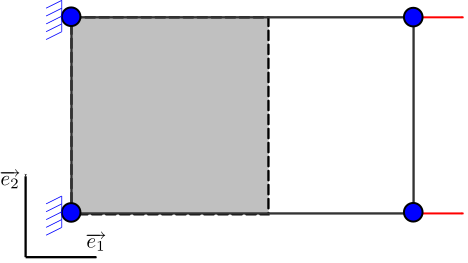
\includegraphics[width=0.5\columnwidth]{Figures/SamplesSingleTensile}
\par\end{centering}
\caption{Numerical model for the one element tensile test\label{fig:Samples!Single!Tensile}}
\end{figure}
 The initial shape of the specimen is $10\,mm\times10\,mm$, the two
left nodes of the element are encastred and a prescribed horizontal
displacement $d=10\,mm$ is applied on the two right nodes of the
same element as illustrated in Figure \ref{fig:Samples!Single!Tensile}.
As we are using an explicit integration scheme, the total simulation
time is set to $t=0.01\,s$. 

All the properties of the constitutive law reported in Table \ref{tab:Samples!JohnsonCookParameters}
are used and the material is assumed to follow the Johnson-Cook behavior
described by equation \ref{eq:Samples!Johnson-Cook}.

Figure \ref{fig:Samples!Single!Tensile-Comparison} shows the comparison
of the DynELA solver results (plotted in red) and the Abaqus numerical
results (plotted in blue) concerning the evolution of the stress components
$\sigma_{11}$, $\sigma_{22}$, $\sigma_{12}$, $\overline{\sigma}$,
$\overline{\varepsilon}^{p}$ and $T$ \versus  the horizontal displacement
of the right edge of the specimen along the horizontal axis. For the
Abaqus model, the exact same mesh has been used. Comparison of Abaqus
and DynELA results is made by averaging the DynELA results on the
$4$ integration points of the element. This has been done because
\DynELA~uses full integrated elements while Abaqus have reduced
integrated elements only but in fact, the DynELA results at the $4$
integration points are the same in this benchmark test.

\begin{figure}[h]
\begin{centering}
\begin{tabular}{cc}
\includegraphics[width=0.45\columnwidth]{Figures/Samples/Element/Tensile_stress_11} & \includegraphics[width=0.45\columnwidth]{Figures/Samples/Element/Tensile_stress_22}\tabularnewline
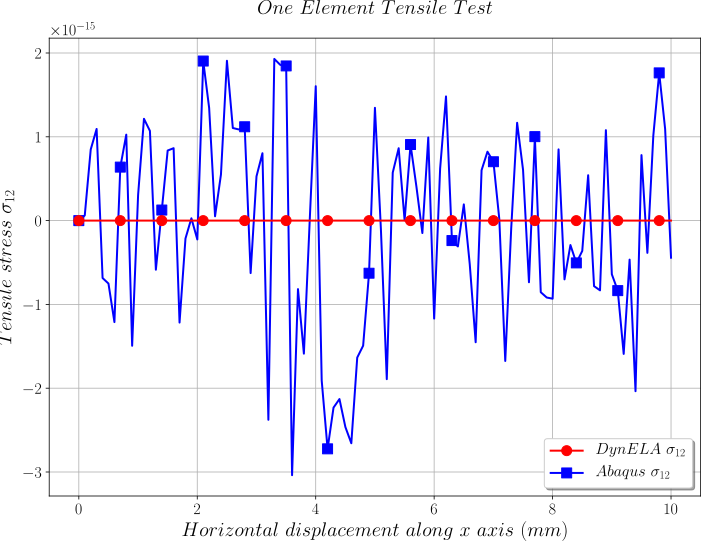
\includegraphics[width=0.45\columnwidth]{Figures/Samples/Element/Tensile_stress_12} & 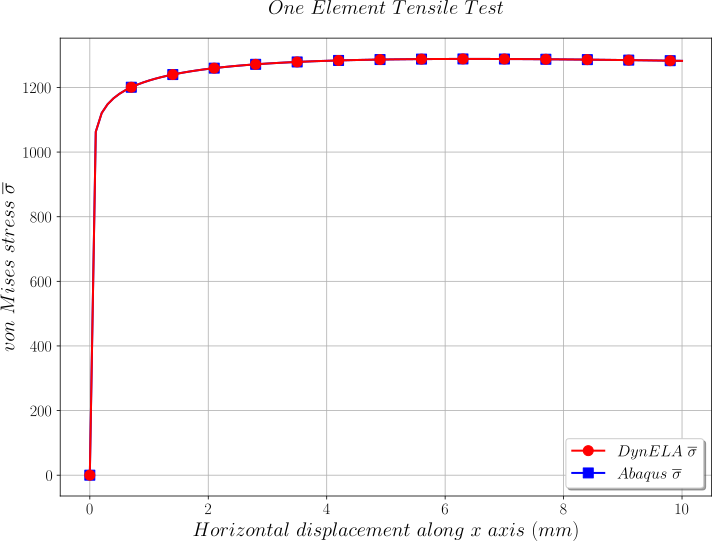
\includegraphics[width=0.45\columnwidth]{Figures/Samples/Element/Tensile_vonMises}\tabularnewline
\includegraphics[width=0.45\columnwidth]{Figures/Samples/Element/Tensile_plasticStrain} & 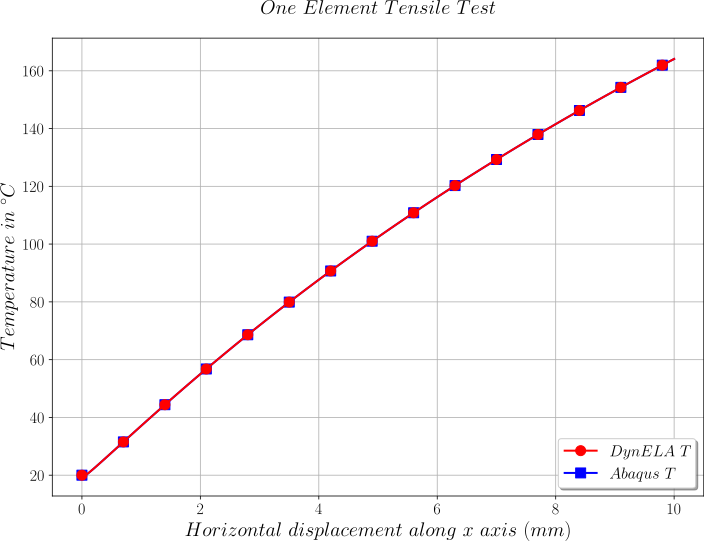
\includegraphics[width=0.45\columnwidth]{Figures/Samples/Element/Tensile_temperature}\tabularnewline
\end{tabular}
\par\end{centering}
\caption{Comparison of numerical and analytical results for the one element
tensile test\label{fig:Samples!Single!Tensile-Comparison}}
\end{figure}
\clearpage

\subsection{Element 3D tensile test}

The uniaxial one element 3D tensile test is a numerical test where
a 3D brick element (with a cubic prescribed shape) is subjected to
radial tensile as presented in figure \ref{fig:Samples!Single!Tensile-3D}.
No boundary condition has been prescribed on the $\overrightarrow{z}$
direction, so that the reduction of the width during the test can
occur. The initial shape of the specimen is $10\,mm\times10\,mm\times10\,mm$
and the the two left nodes of the element are restrained for their
displacements along the $\overrightarrow{x}$ and $\overrightarrow{y}$
directions and a prescribed horizontal displacement $d=10\,mm$ is
applied on the two right nodes of the same element as illustrated
in Figure \ref{fig:Samples!Single!Tensile-3D}. As we are using an
explicit integration scheme, the total simulation time is set to $t=0.01\,s$.
\begin{figure}[h]
\begin{centering}
\includegraphics[width=0.5\columnwidth]{Figures/SamplesSingleTensile3D}
\par\end{centering}
\caption{Numerical model for the one element tensile test\label{fig:Samples!Single!Tensile-3D}}
\end{figure}

All the properties of the constitutive law reported in Table \ref{tab:Samples!JohnsonCookParameters}
are used and the material is assumed to follow the Johnson-Cook behavior
described by equation \ref{eq:Samples!Johnson-Cook}.

Figure \ref{fig:Samples!Single!Tensile-Comparison-3D} shows the comparison
of the DynELA solver results (plotted in red) and the Abaqus numerical
results (plotted in blue) concerning the evolution of the stress components
$\sigma_{11}$, $\sigma_{22}$, $\sigma_{12}$, $\overline{\sigma}$,
$\overline{\varepsilon}^{p}$ and $T$ \versus  the horizontal displacement
of the right edge of the specimen along the horizontal axis. For the
Abaqus model, the exact same mesh has been used. Comparison of Abaqus
and DynELA results is made by averaging the DynELA and the Abaqus
results on the $8$ integration points of the element.

\begin{figure}[h]
\begin{centering}
\begin{tabular}{cc}
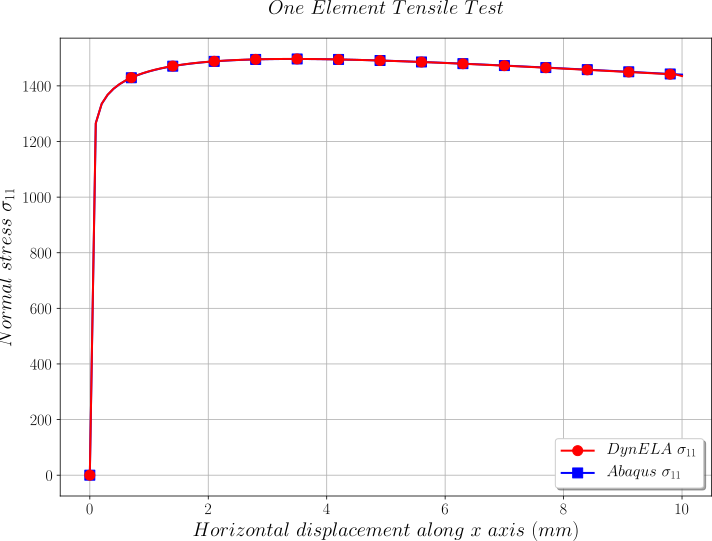
\includegraphics[width=0.45\columnwidth]{Figures/Samples/Element/Tensile3D_stress_11} & 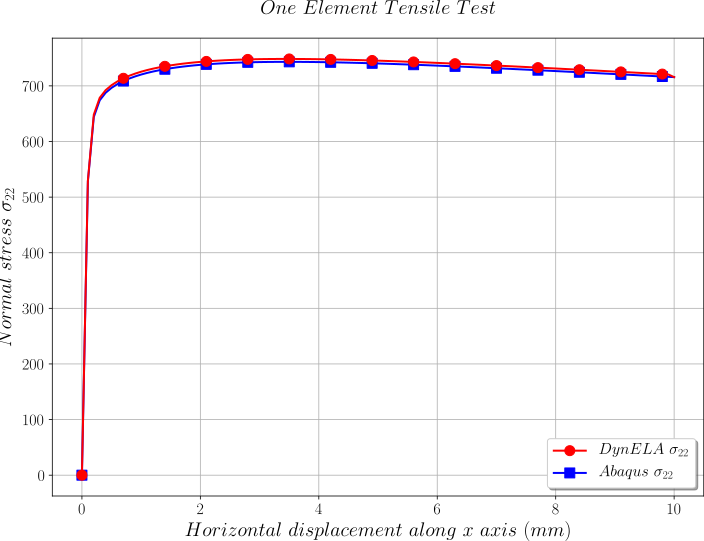
\includegraphics[width=0.45\columnwidth]{Figures/Samples/Element/Tensile3D_stress_22}\tabularnewline
\includegraphics[width=0.45\columnwidth]{Figures/Samples/Element/Tensile3D_stress_12} & \includegraphics[width=0.45\columnwidth]{Figures/Samples/Element/Tensile3D_vonMises}\tabularnewline
\includegraphics[width=0.45\columnwidth]{Figures/Samples/Element/Tensile3D_plasticStrain} & \includegraphics[width=0.45\columnwidth]{Figures/Samples/Element/Tensile3D_temperature}\tabularnewline
\end{tabular}
\par\end{centering}
\caption{Comparison of numerical and analytical results for the 3D one element
tensile test\label{fig:Samples!Single!Tensile-Comparison-3D}}
\end{figure}


\subsection{Element radial tensile test}

The uniaxial one element radial tensile test is a numerical test where
an axisymmetric element (with a square prescribed shape) is subjected
to pure radial tensile as presented in figure \ref{fig:Samples!Single!Tensile}.
The initial shape of the specimen is $10\,mm\times10\,mm$ and the
the two left nodes of the element are encastred and a prescribed horizontal
displacement $d=10\,mm$ is applied on the two right nodes of the
same element as illustrated in Figure \ref{fig:Samples!Single!Tensile}.
As we are using an explicit integration scheme, the total simulation
time is set to $t=0.01\,s$. 

All the properties of the constitutive law reported in Table \ref{tab:Samples!JohnsonCookParameters}
are used and the material is assumed to follow the Johnson-Cook behavior
described by equation \ref{eq:Samples!Johnson-Cook}. 

Figure \ref{fig:Samples!Single!Radial-Comparison} shows the comparison
of the DynELA solver results (plotted in red) and the Abaqus numerical
results (plotted in blue) concerning the evolution of the stress components
$\sigma_{11}$, $\sigma_{22}$, $\sigma_{12}$, $\overline{\sigma}$,
$\overline{\varepsilon}^{p}$ and $T$ \versus  the horizontal displacement
of the right edge of the specimen along the horizontal axis. Again,
comparison of Abaqus and DynELA results is made by averaging the DynELA
results on the $4$ integration points of the element because \DynELA~uses
full integrated elements while Abaqus have reduced integrated elements
only but in fact, the DynELA results at the $4$ integration points
are the same in this benchmark test. 

\begin{figure}[h]
\begin{centering}
\begin{tabular}{cc}
\includegraphics[width=0.45\columnwidth]{Figures/Samples/Element/Radial_stress_11} & \includegraphics[width=0.45\columnwidth]{Figures/Samples/Element/Radial_stress_22}\tabularnewline
\includegraphics[width=0.45\columnwidth]{Figures/Samples/Element/Radial_stress_12} & \includegraphics[width=0.45\columnwidth]{Figures/Samples/Element/Radial_vonMises}\tabularnewline
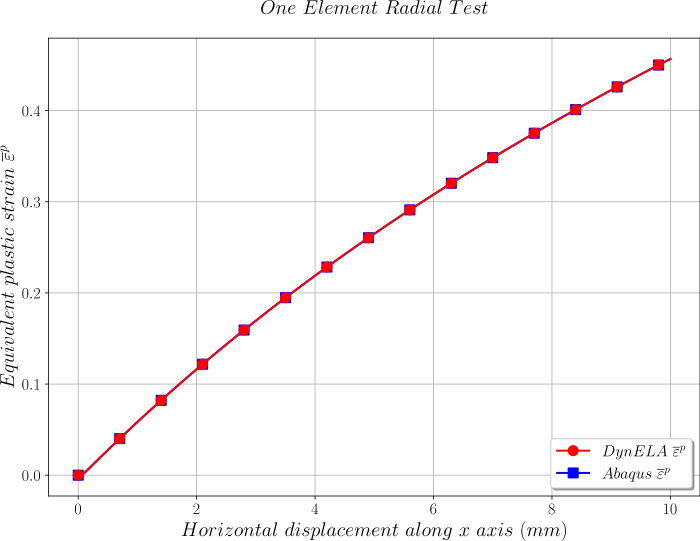
\includegraphics[width=0.45\columnwidth]{Figures/Samples/Element/Radial_plasticStrain} & 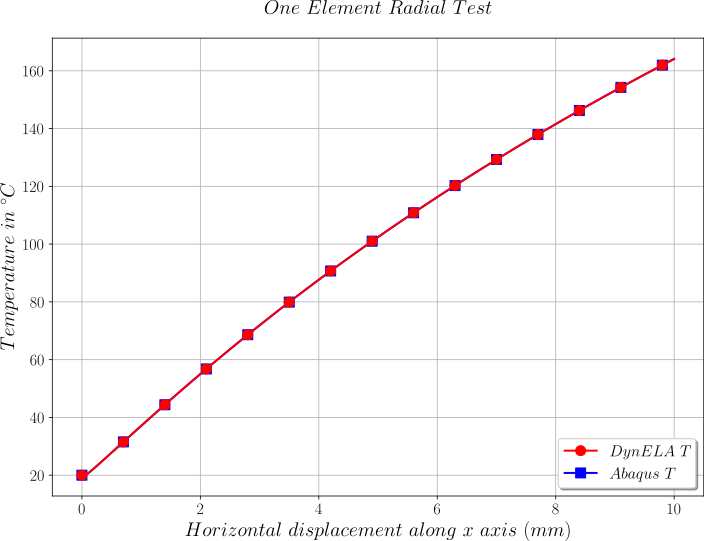
\includegraphics[width=0.45\columnwidth]{Figures/Samples/Element/Radial_temperature}\tabularnewline
\end{tabular}
\par\end{centering}
\caption{Comparison of numerical and analytical results for the one element
radial tensile test\label{fig:Samples!Single!Radial-Comparison}}
\end{figure}
\clearpage

\subsection{Element radial torus test}

The uniaxial one element torus tensile test is a numerical test where
an axisymmetric element (with a square prescribed shape) is subjected
to radial tensile as presented in figure \ref{fig:Samples!Single!Torus}.
\begin{figure}[h]
\begin{centering}
\includegraphics[width=0.5\columnwidth]{Figures/SamplesSingleTorus}
\par\end{centering}
\caption{Numerical model for the one element torus test\label{fig:Samples!Single!Torus}}
\end{figure}
 The difference with the previous test is that the left edge of the
specimen in not aligned with the symmetry axis, the radial coordinate
of the left edge is $r=10\,mm$. The initial shape of the specimen
is $10\,mm\times10\,mm$ and a prescribed horizontal displacement
$d=10\,mm$ is applied on the two left nodes of the element as illustrated
in Figure \ref{fig:Samples!Single!Torus}. As we are using an explicit
integration scheme, the total simulation time is set to $t=0.01\,s$.
All the properties of the constitutive law reported in Table \ref{tab:Samples!JohnsonCookParameters}
are used and the material is assumed to follow the Johnson-Cook behavior
described by equation \ref{eq:Samples!Johnson-Cook}.

As a global comparison, Figure \ref{fig:Samples!Single!Torus-Comparison-ux}
show the comparison of the right edge displacement \versus the left
edge displacement for both the DynELA and the Abaqus simulations.
\begin{figure}[h]
\begin{centering}
\includegraphics[width=0.5\columnwidth]{Figures/Samples/Element/Torus_dispX}
\par\end{centering}
\caption{Comparison of the right edge displacement for the one element torus
test\label{fig:Samples!Single!Torus-Comparison-ux}}
\end{figure}

Figure \ref{fig:Samples!Single!Torus-Comparison} shows the comparison
of the DynELA solver results (plotted in red) and the Abaqus numerical
results (plotted in blue) concerning the evolution of the stress components
$\sigma_{11}$, $\sigma_{22}$, $\sigma_{12}$, $\overline{\sigma}$,
$\overline{\varepsilon}^{p}$ and $T$ \versus  the horizontal displacement
of the right edge of the specimen along the horizontal axis. As the
Abaqus software only provides under-integrated elements, we are using
a $2\times2$ elements mesh for the Abaqus model, as presented in
Figure \ref{fig:Samples!Single!Torus-Abaqus}, to compare the results.
On abaqus, the mean value of the results of the $4$ elements is computed
and compared to the mean value of the $4$ integration points of the
DynELA simulation.
\begin{figure}[h]
\begin{centering}
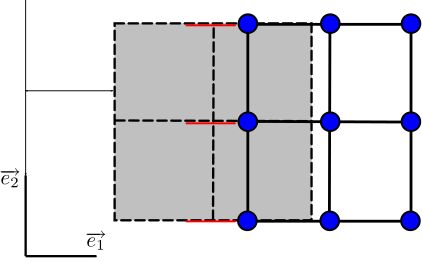
\includegraphics[width=0.5\columnwidth]{Figures/SamplesSingleTorusAbaqus}
\par\end{centering}
\caption{Numerical model for the one element torus test under Abaqus\label{fig:Samples!Single!Torus-Abaqus}}
\end{figure}

\begin{figure}[h]
\begin{centering}
\begin{tabular}{cc}
\includegraphics[width=0.45\columnwidth]{Figures/Samples/Element/Torus_stress_11} & \includegraphics[width=0.45\columnwidth]{Figures/Samples/Element/Torus_stress_22}\tabularnewline
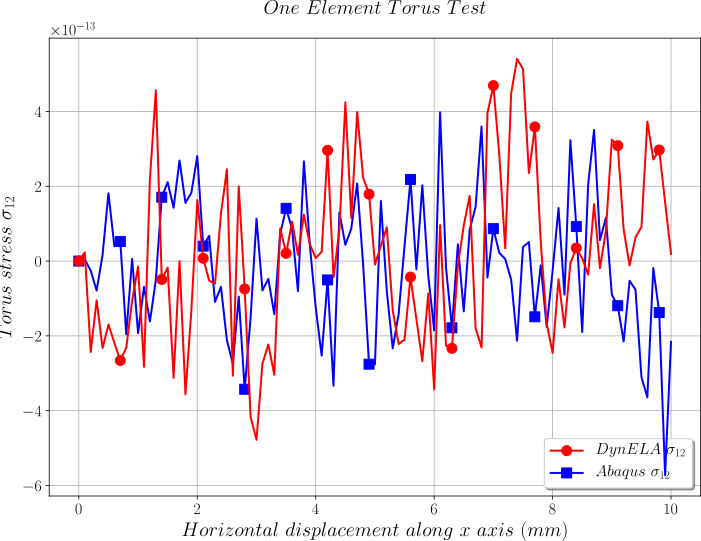
\includegraphics[width=0.45\columnwidth]{Figures/Samples/Element/Torus_stress_12} & 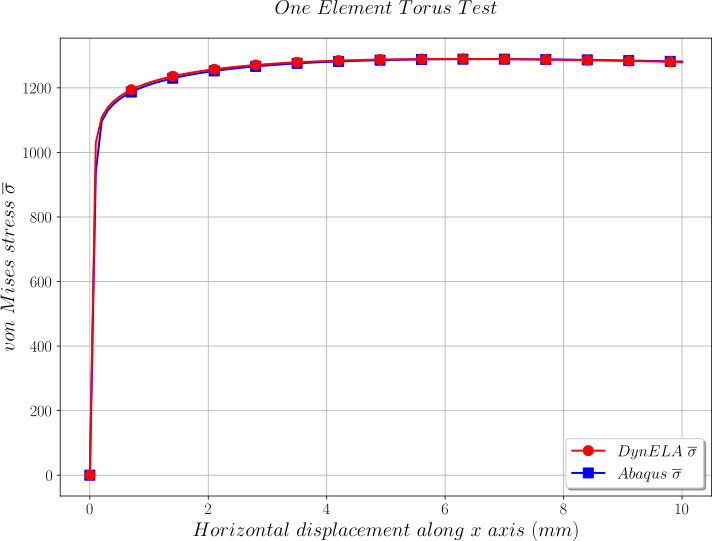
\includegraphics[width=0.45\columnwidth]{Figures/Samples/Element/Torus_vonMises}\tabularnewline
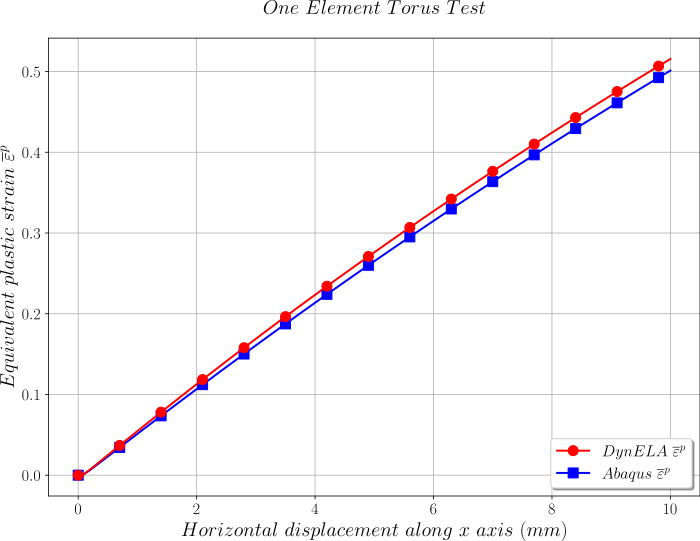
\includegraphics[width=0.45\columnwidth]{Figures/Samples/Element/Torus_plasticStrain} & 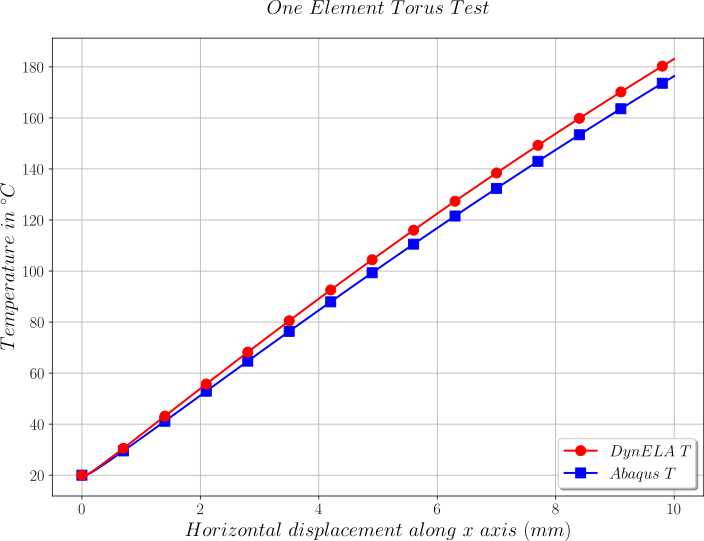
\includegraphics[width=0.45\columnwidth]{Figures/Samples/Element/Torus_temperature}\tabularnewline
\end{tabular}
\par\end{centering}
\caption{Comparison of numerical results for the one element torus tensile
test\label{fig:Samples!Single!Torus-Comparison}}
\end{figure}
\clearpage

\section{Uniaxial one element shear test}

The uniaxial one element shear test is a numerical test where an element
(with a square prescribed shape) is subjected to pure shear test as
presented in figure \ref{fig:Samples!Single!Shear}.
\begin{figure}[h]
\begin{centering}
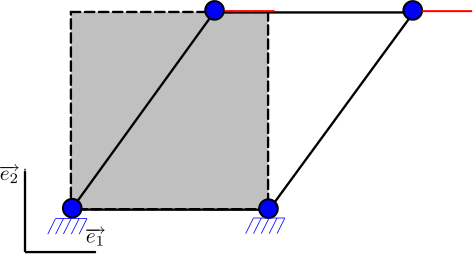
\includegraphics[width=0.5\columnwidth]{Figures/SamplesSingleShear}
\par\end{centering}
\caption{Numerical model for the one element shear test\label{fig:Samples!Single!Shear}}
\end{figure}
 The initial shape of the specimen is $10\,mm\times10\,mm$ and the
the two bottom nodes of the element are encastred and a prescribed
horizontal displacement $d=100\,mm$ is applied on the two upper nodes
of the same element as illustrated in Figure \ref{fig:Samples!Single!Shear}.
As we are using an explicit integration scheme, the total simulation
time is set to $t=0.01\,s$. Mechanical properties of the material
are reported in Table \ref{tab:Samples!JohnsonCookParameters}. 

Comparison of Abaqus and DynELA results is made by averaging the DynELA
results on the $4$ integration points of the element. This has been
done because \DynELA~uses full integrated elements while Abaqus
have reduced integrated elements only but in fact, the DynELA results
at the $4$ integration points are the same in this benchmark test.

\subsection{Elastic case}

In this case, only the elastic properties of the constitutive law
reported in Table \ref{tab:Samples!JohnsonCookParameters} are used
and the material is assumed to be hyper-elastic. As we are using a
Jaumann objective rate within the \DynELA, one can obtain, using
an analytical development, the following results for the proposed
case:
\begin{equation}
\Sig=G\left[\begin{array}{ccc}
1-\cos e & \sin e & 0\\
 & \cos e-1 & 0\\
sym &  & 0
\end{array}\right],
\end{equation}
where $G=\mu=\frac{E}{2(1+\nu)}$ is the shear modulus of the material
and $e$ is the elongation along the horizontal axis with $e_{max}=10$
conforming to the prescribed boundaries conditions. Figure \ref{fig:Samples!Single!Shear-Elastic-Comparison}
shows the comparison of the DynELA solver results (plotted in red)
and both the analytical (plotted in blue) and the Abaqus numerical
results (plotted in green) concerning the evolution of the stress
components $\sigma_{11}$, $\sigma_{22}$, $\sigma_{12}$ and $\overline{\sigma}$
\versus  the horizontal displacement of the top edge of the specimen
along the horizontal axis. A perfect match between all those results
can be seen from this later.

\begin{figure}[h]
\begin{centering}
\begin{tabular}{cc}
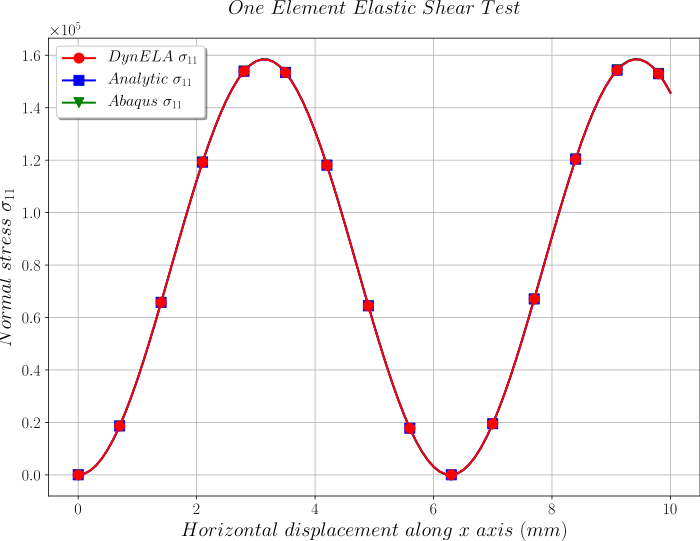
\includegraphics[width=0.45\columnwidth]{Figures/Samples/Element/Shear-Elastic_stress_11} & \includegraphics[width=0.45\columnwidth]{Figures/Samples/Element/Shear-Elastic_stress_22}\tabularnewline
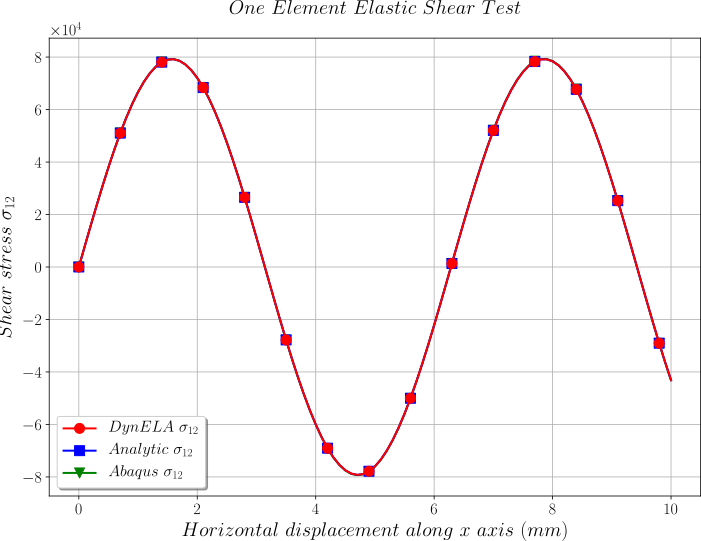
\includegraphics[width=0.45\columnwidth]{Figures/Samples/Element/Shear-Elastic_stress_12} & \includegraphics[width=0.45\columnwidth]{Figures/Samples/Element/Shear-Elastic_vonMises}\tabularnewline
\end{tabular}
\par\end{centering}
\caption{Comparison of numerical and analytical results for the one element
elastic shear test\label{fig:Samples!Single!Shear-Elastic-Comparison}}
\end{figure}
\clearpage

\subsection{Johnson-Cook plastic behaviour}

In this case, all the properties of the constitutive law reported
in Table \ref{tab:Samples!JohnsonCookParameters} are used and the
material is assumed to follow the Johnson-Cook behavior described
by equation \ref{eq:Samples!Johnson-Cook}. Figure \ref{fig:Samples!Single!Shear-Comparison}
shows the comparison of the DynELA solver results (plotted in red)
and the Abaqus numerical results (plotted in blue) concerning the
evolution of the stress components $\sigma_{11}$, $\sigma_{22}$,
$\sigma_{12}$, $\overline{\sigma}$, $\overline{\varepsilon}^{p}$
and $T$ \versus  the horizontal displacement of the top edge of
the specimen along the horizontal axis.

\begin{figure}[h]
\begin{centering}
\begin{tabular}{cc}
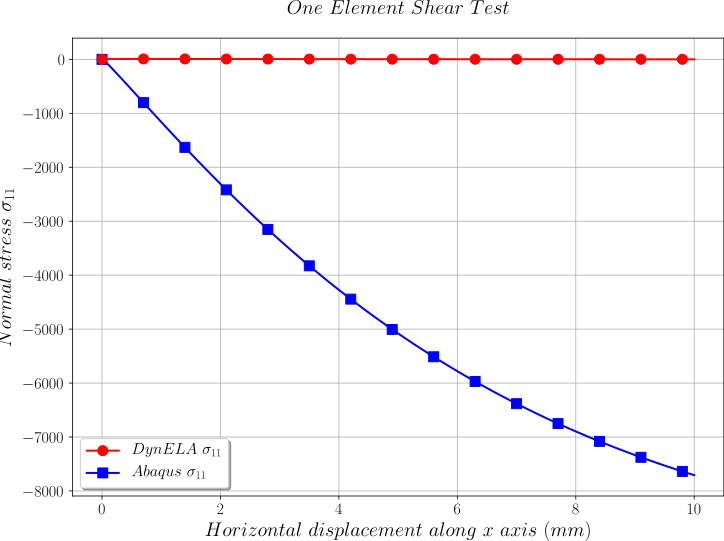
\includegraphics[width=0.45\columnwidth]{Figures/Samples/Element/Shear-Plastic_stress_11} & \includegraphics[width=0.45\columnwidth]{Figures/Samples/Element/Shear-Plastic_stress_22}\tabularnewline
\includegraphics[width=0.45\columnwidth]{Figures/Samples/Element/Shear-Plastic_stress_12} & \includegraphics[width=0.45\columnwidth]{Figures/Samples/Element/Shear-Plastic_vonMises}\tabularnewline
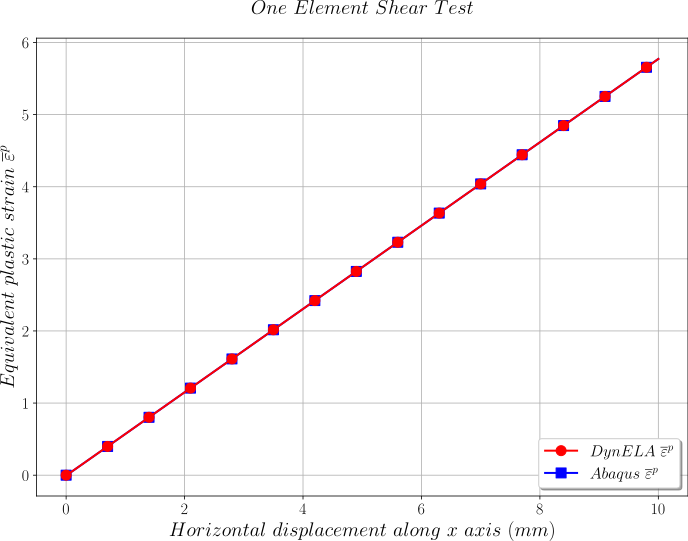
\includegraphics[width=0.45\columnwidth]{Figures/Samples/Element/Shear-Plastic_plasticStrain} & \includegraphics[width=0.45\columnwidth]{Figures/Samples/Element/Shear-Plastic_temperature}\tabularnewline
\end{tabular}
\par\end{centering}
\caption{Comparison of numerical and analytical results for the one element
shear test\label{fig:Samples!Single!Shear-Comparison}}
\end{figure}




\chapter{DynELA plasticity sample cases}

\startcontents[chapters]
\printmyminitoc[1]\LETTRINE{T}his chapter deals with some numerical applications of
the \DynELA~for plasticity applications in 2D, axi-symmetric and
3D cases. In the subsequent tests, if not specified, a Johnson-Cook
constitutive law is used to model the behavior of the material. The
Johnson-Cook hardening flow law is probably the most widely used flow
law for the simulation of high strain rate deformation processes taking
into account plastic strain, plastic strain rate and temperature effects.
Since a lot of efforts have been made in the past to identify the
constitutive flow law parameters for many materials, it is implemented
in numerous Finite Element codes such as Abaqus \cite{abaqus20146}.
The general formulation of the Johnson-Cook law $\sigma^{y}(\overline{\varepsilon}^{p},\stackrel{\bullet}{\overline{\varepsilon}^{p}},T)$
is given by the following equation:

\begin{equation}
\sigma^{y}=\left(A+B\overline{\varepsilon}^{p^{n}}\right)\left[1+C\ln\left(\frac{\stackrel{\bullet}{\overline{\varepsilon}^{p}}}{\stackrel{\bullet}{\overline{\varepsilon}_{0}}}\right)\right]\left[1-\left(\frac{T-T_{0}}{T_{m}-T_{0}}\right)^{m}\right]\label{eq:Samples!Johnson-Cook}
\end{equation}
where $\stackrel{\bullet}{\overline{\varepsilon}_{0}}$ is the reference
strain rate, $T_{0}$ and $T_{m}$ are the reference temperature and
the melting temperature of the material respectively and $A$, $B$,
$C$, $n$ and $m$ are the five constitutive flow law parameters.
A 42CrMo4 steel following the Johnson-Cook behavior law has been selected
for all those tests, and material properties are reported in Table
\ref{tab:Samples!JohnsonCookParameters}.

\begin{table}[h]
\begin{center}\begin{tcolorbox}[width=.75\textwidth,myTab,tabularx={C|C|C|C|C|C|C}]
$E$ & $\nu$ & $A$ & $B$ & $C$ & $n$ & $m$ \\
\small{($Gpa$)} &  & \small{($MPa$)} & \small{($MPa$)} &  &  & \\ \hline
$206.9$ & $0.3$ & $806$ & $614$ & $0.0089$ & $0.168$ & $1.1$ \\ \hline\hline
$\rho$ & $\lambda$ & $C_{p}$ & $\eta$ & $\stackrel{\bullet}{\overline{\varepsilon}_{0}}$ & $T_{0}$ & $T_{m}$ \\
\small{$(kg/m^{3})$} & \small{$(W/m^{\circ}C)$} & \small{$(J/Kg^{\circ}C)$} & & \small{$(s^{-1})$} & \small{$(^{\circ}C)$} & \small{$(^{\circ}C)$} \\ \hline
$7830$ & $34.0$ & $460$ & $0.9$ & $1.0$ & $20$ & $1540$
\end{tcolorbox}\end{center}\caption{Material parameters of the Johnson-Cook behavior for the numerical
tests\label{tab:Samples!JohnsonCookParameters}}
\end{table}


\section{Necking of a circular bar}

\subsection{Axisymmetric Bar Necking}

The necking of a circular bar test is useful to evaluate the performance
of VUMAT subroutine for materials in presence of plasticity and large
deformation \cite{ponthot_unified_2002, j_c_simo_computational_1998}. Because of the symmetric
structure, an axisymmetric quarter model of the specimen is established.
Dimensions of the specimen are reported in Figure \ref{fig:Samples!Plasticity!NeckingAxi}.
The loading is realized through an imposed total displacement of $7\,mm$
along the $\overrightarrow{z}$ axis on the left side of the specimen
while the radial displacement of the same edge is supposed to remain
zero. On the opposite side the axial displacement is restrained while
the radial displacement is free. The mesh consists of $400$ CAX4RT
elements with a refined zone of $200$ elements on the right side
on $1/3$ of the total height. Again, the total simulation time is
set to $t=0.01\,s$ because of the explicit integration scheme adopted. 

\begin{figure}[h]
\begin{centering}
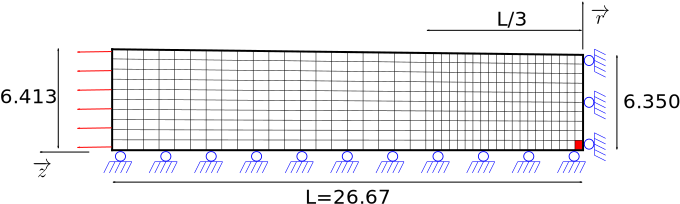
\includegraphics[width=0.75\columnwidth]{Figures/BarNecking}
\par\end{centering}
\caption{Numerical model for the necking of a circular bar\label{fig:Samples!Plasticity!NeckingAxi}}
\end{figure}

Figures \ref{fig:Samples!Plasticity!BarAxi-temp-contour} and \ref{fig:Samples!Plasticity!BarAxi-mises-contour}
shows the temperature $T$ and the von Mises stress $\overline{\sigma}$
contourplots of the deformed rod for both the \DynELA~and Abaqus.
The distributions of the temperatures and stresses are almost the
same for both models. The maximum temperature $T$ is located into
the center element of the model (the red element in Figure \ref{fig:Samples!Plasticity!NeckingAxi})
and the models give quite the same results as reported in Table \ref{tab:Samples!Plasticity!BarAxi-comparison}
for $\overline{\varepsilon}^{p}$, $T$ and the final dimensions of
the specimen $D_{f}$ (final diameter of the necking zone). 

Figure \ref{fig:Samples!Plasticity!BarAxi-comparison} shows the evolution
of the the final dimensions of the specimen $L_{f}$ (final length)
and $R_{f}$ (final radius of the impacting face), the equivalent
plastic strain $\overline{\varepsilon}^{p}$, the temperature $T$,
the von Mises stress $\overline{\sigma}$ and the timeStep $\Delta t$
for the different models for the element at the center of the impacting
face (the red element in Figure \ref{fig:Samples!Plasticity!NeckingAxi}). 

As reported in this figure and according to the results presented
in Table \ref{tab:Samples!Plasticity!BarAxi-comparison}, a quite
good agreement between the results is obtained.

\begin{figure}[h]
\begin{centering}
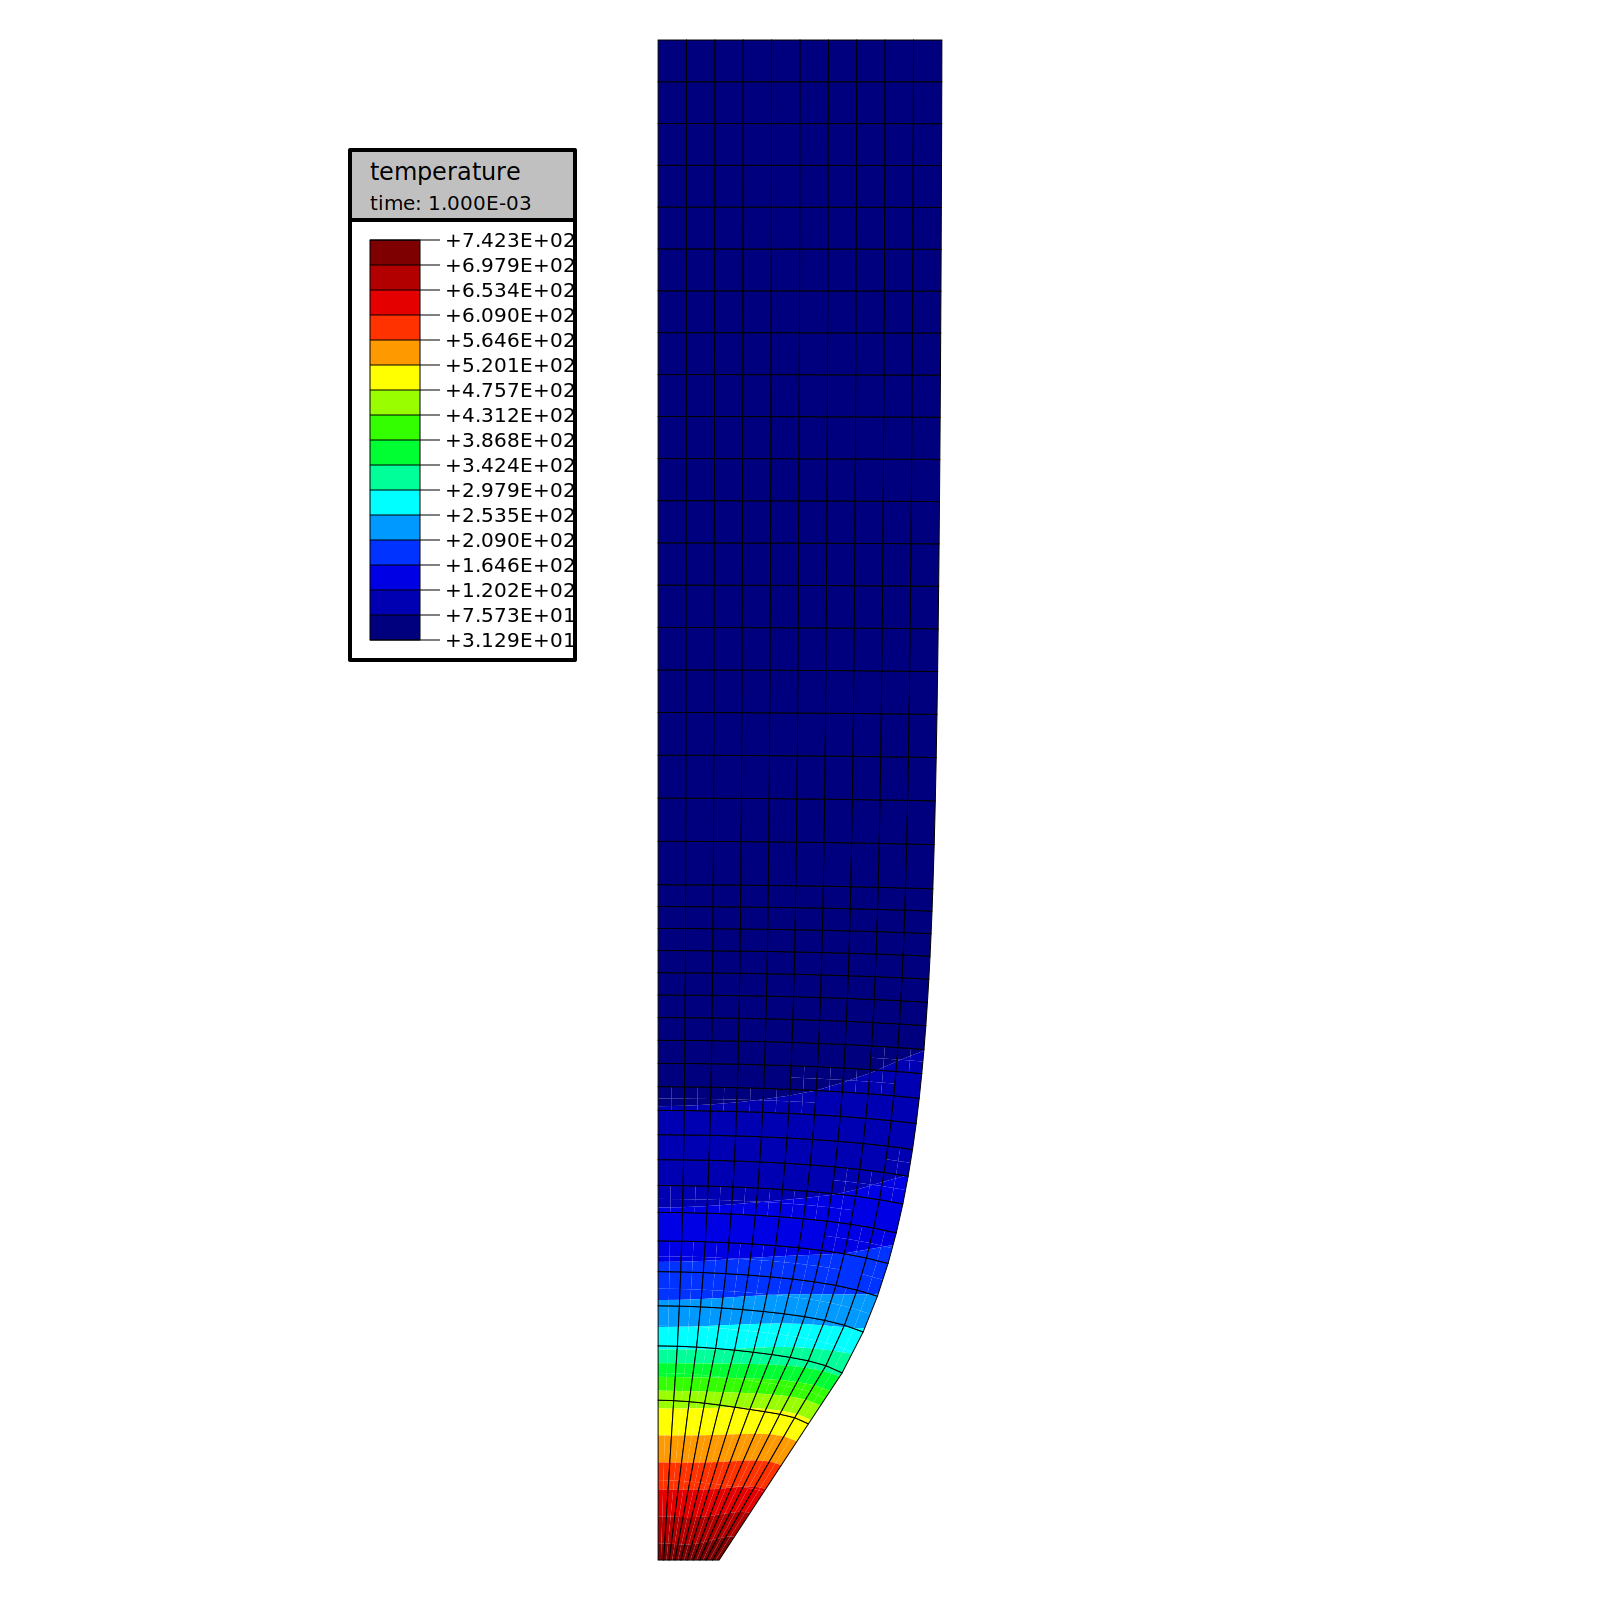
\includegraphics[height=0.5\columnwidth]{Figures/Samples/Plasticity/BarNecking_temperatureCP}\hspace*{3cm}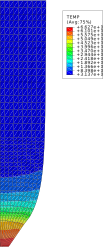
\includegraphics[height=0.5\columnwidth]{Figures/Samples/Plasticity/BarNecking-Abaqus_temperature}
\par\end{centering}
\caption{Temperature $T$ contourplot for the necking of a circular bar (DynELA
left and Abaqus right)\label{fig:Samples!Plasticity!BarAxi-temp-contour}}
\end{figure}

\begin{figure}[h]
\begin{centering}
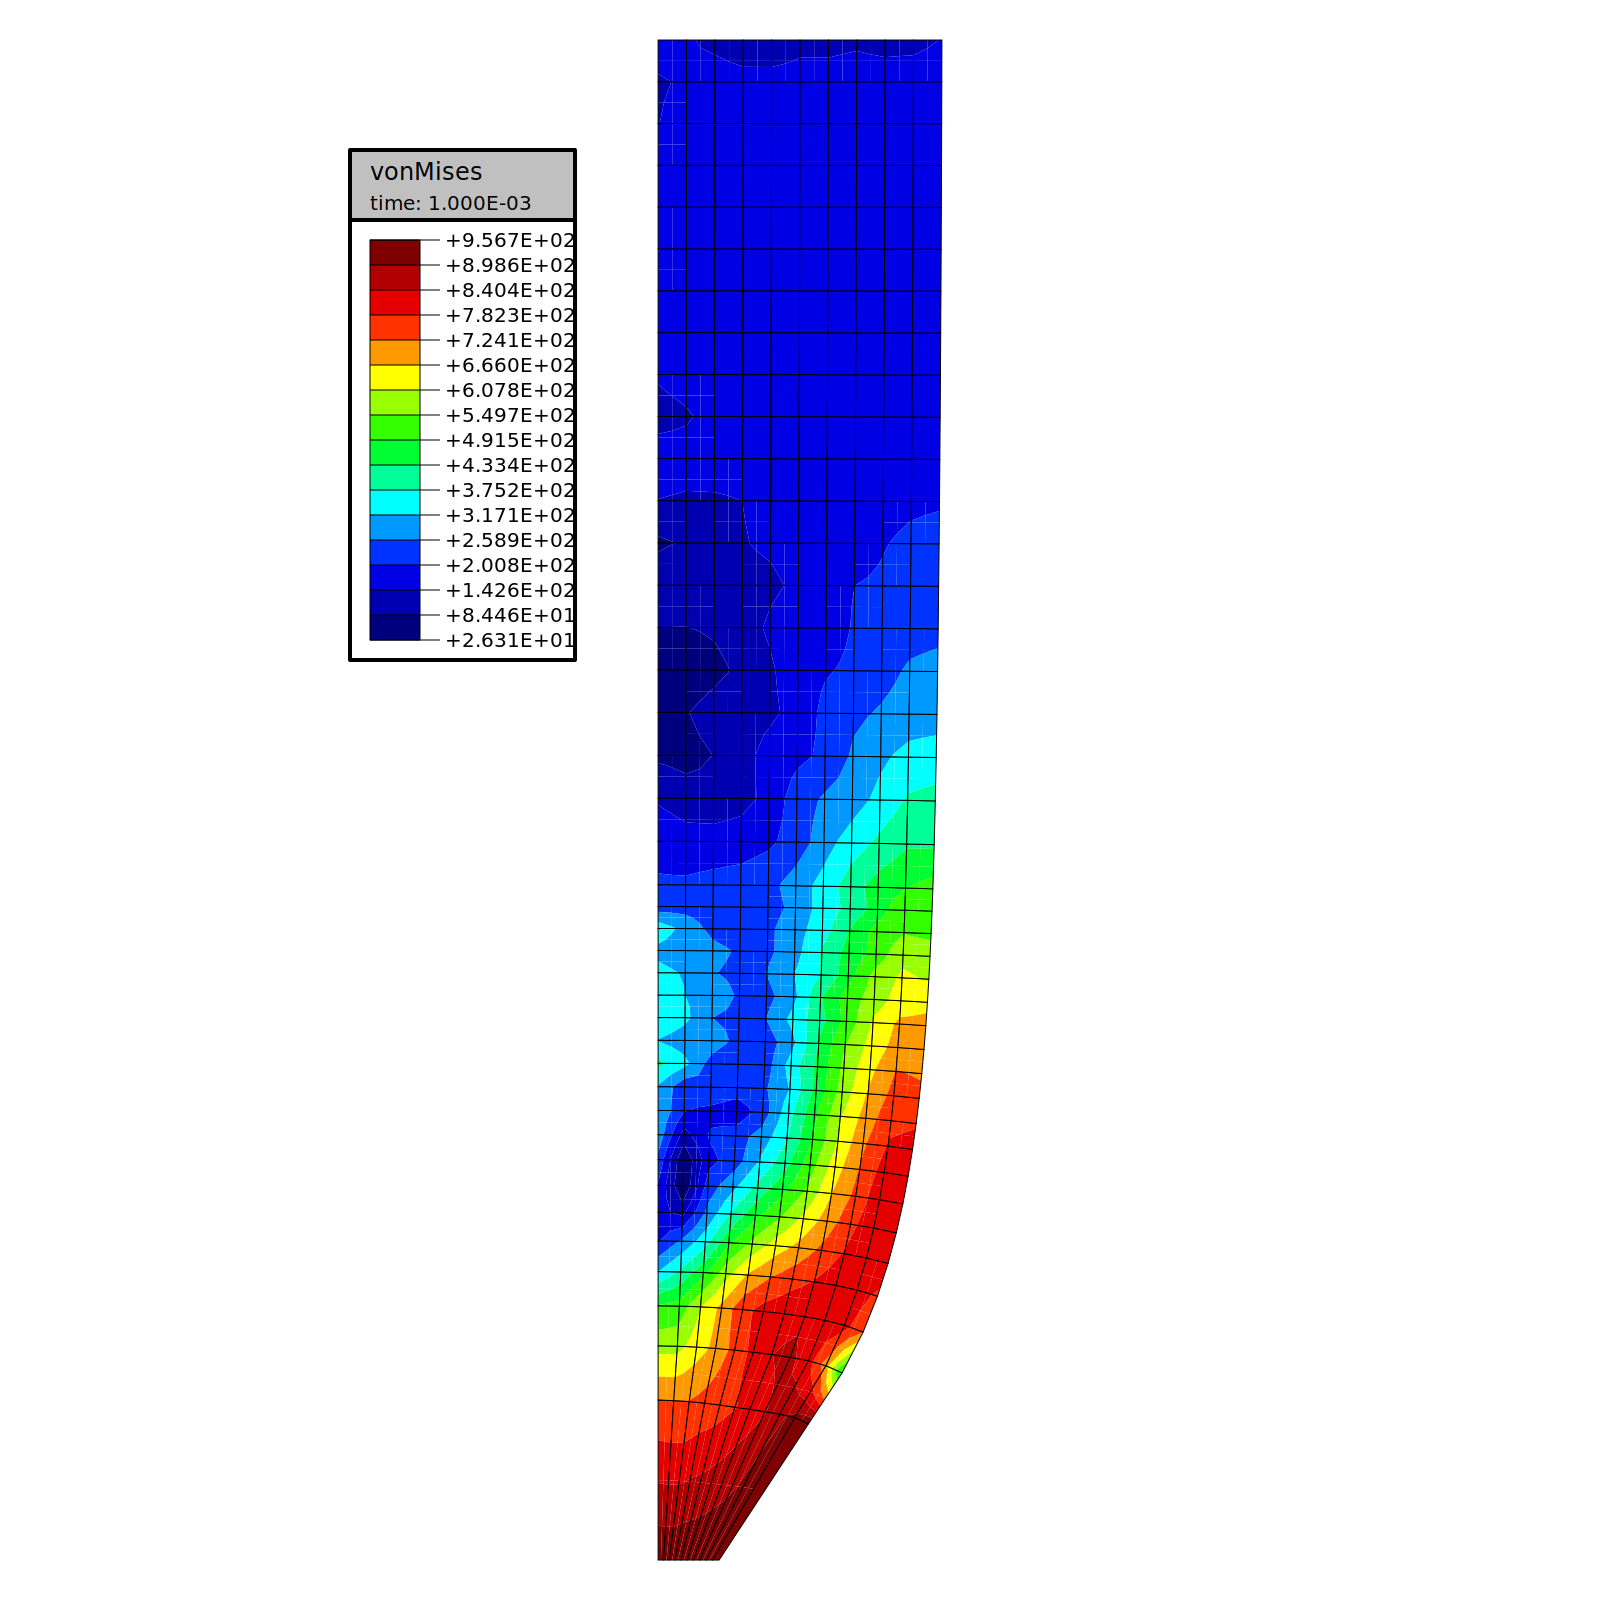
\includegraphics[height=0.5\columnwidth]{Figures/Samples/Plasticity/BarNecking_vonMisesCP}\hspace*{3cm}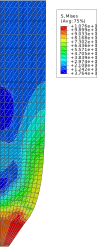
\includegraphics[height=0.5\columnwidth]{Figures/Samples/Plasticity/BarNecking-Abaqus_vonMises}
\par\end{centering}
\caption{von Mises stress $\overline{\sigma}$ contourplot for the necking
of a circular bar (DynELA left and Abaqus right)\label{fig:Samples!Plasticity!BarAxi-mises-contour}}
\end{figure}

\begin{table}[h]
\begin{center}\begin{tcolorbox}[width=.75\textwidth,myTab,tabularx={C|C|C|C}]
code & $D_f$ & $T$ & $\overline{\varepsilon}^{p}$ \\
 & \small{($mm$)} & \small{($^{\circ}C$)} & \\ \hline\hline
DynELA & $2.71$ & $642.78$ & $2.07$ \\ \hline
Abaqus & $2.35$ & $658.91$ & $2.12$
\end{tcolorbox}\end{center}\caption{Comparison of numerical results for the necking of a circular bar
test\label{tab:Samples!Plasticity!BarAxi-comparison}}
\end{table}

\begin{figure}[h]
\begin{centering}
\begin{tabular}{cc}
\includegraphics[width=0.45\columnwidth]{Figures/Samples/Plasticity/BarNecking_radius} & 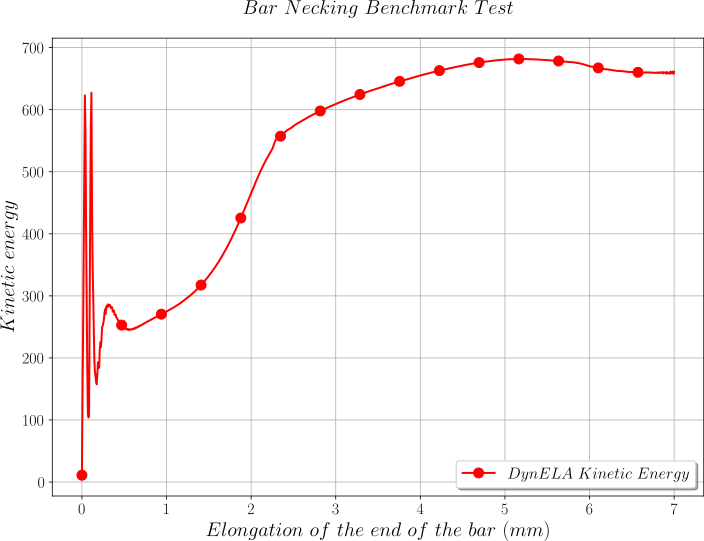
\includegraphics[width=0.45\columnwidth]{Figures/Samples/Plasticity/BarNecking_kineticEnergy}\tabularnewline
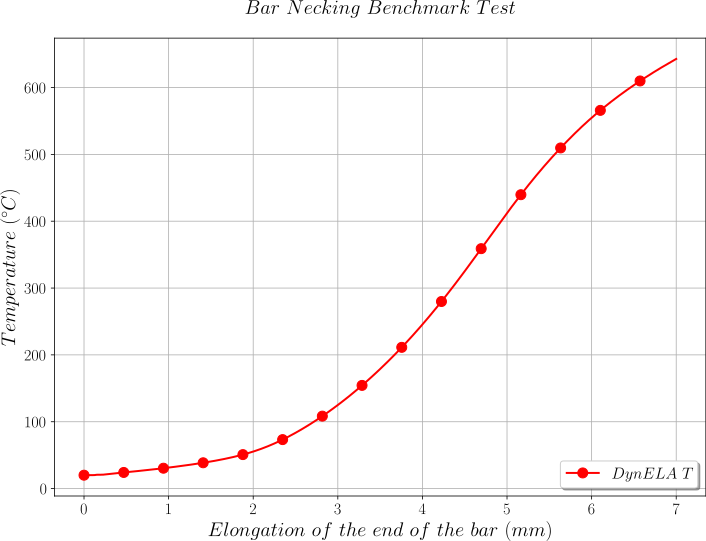
\includegraphics[width=0.45\columnwidth]{Figures/Samples/Plasticity/BarNecking_temperature} & \includegraphics[width=0.45\columnwidth]{Figures/Samples/Plasticity/BarNecking_plasticStrain}\tabularnewline
\includegraphics[width=0.45\columnwidth]{Figures/Samples/Plasticity/BarNecking_vonMises} & \includegraphics[width=0.45\columnwidth]{Figures/Samples/Plasticity/BarNecking_timeStep}\tabularnewline
\end{tabular}
\par\end{centering}
\caption{Comparison of numerical and analytical results necking of a circular
bar test\label{fig:Samples!Plasticity!BarAxi-comparison}}
\end{figure}




\chapter{DynELA impact sample cases}

\startcontents[chapters]
\printmyminitoc[1]\LETTRINE{T}his chapter deals with some numerical applications of
the \Dynela~for impact applications in 2D, axi-symmetric and 3D
cases. In the subsequent tests, if not specified, a Johnson-Cook constitutive
law is used to model the behavior of the material. The Johnson-Cook
hardening flow law is probably the most widely used flow law for the
simulation of high strain rate deformation processes taking into account
plastic strain, plastic strain rate and temperature effects. Since
a lot of efforts have been made in the past to identify the constitutive
flow law parameters for many materials, it is implemented in numerous
Finite Element codes such as Abaqus \cite{abaqus20146}. The general
formulation of the Johnson-Cook law $\sigma^{y}(\overline{\varepsilon}^{p},\stackrel{\bullet}{\overline{\varepsilon}^{p}},T)$
is given by the following equation:

\begin{equation}
\sigma^{y}=\left(A+B\overline{\varepsilon}^{p^{n}}\right)\left[1+C\ln\left(\frac{\stackrel{\bullet}{\overline{\varepsilon}^{p}}}{\stackrel{\bullet}{\overline{\varepsilon}_{0}}}\right)\right]\left[1-\left(\frac{T-T_{0}}{T_{m}-T_{0}}\right)^{m}\right]\label{eq:Samples!Johnson-Cook}
\end{equation}
where $\stackrel{\bullet}{\overline{\varepsilon}_{0}}$ is the reference
strain rate, $T_{0}$ and $T_{m}$ are the reference temperature and
the melting temperature of the material respectively and $A$, $B$,
$C$, $n$ and $m$ are the five constitutive flow law parameters.
A 42CrMo4 steel following the Johnson-Cook behavior law has been selected
for all those tests, and material properties are reported in Table
\ref{tab:Samples!JohnsonCookParameters}.

\begin{table}[h]
\begin{center}\begin{tcolorbox}[width=.75\textwidth,myTab,tabularx={C|C|C|C|C|C|C}]
$E$ & $\nu$ & $A$ & $B$ & $C$ & $n$ & $m$ \\
\small{($Gpa$)} &  & \small{($MPa$)} & \small{($MPa$)} &  &  & \\ \hline
$206.9$ & $0.3$ & $806$ & $614$ & $0.0089$ & $0.168$ & $1.1$ \\ \hline\hline
$\rho$ & $\lambda$ & $C_{p}$ & $\eta$ & $\stackrel{\bullet}{\overline{\varepsilon}_{0}}$ & $T_{0}$ & $T_{m}$ \\
\small{$(kg/m^{3})$} & \small{$(W/m^{\circ}C)$} & \small{$(J/Kg^{\circ}C)$} & & \small{$(s^{-1})$} & \small{$(^{\circ}C)$} & \small{$(^{\circ}C)$} \\ \hline
$7830$ & $34.0$ & $460$ & $0.9$ & $1.0$ & $20$ & $1540$
\end{tcolorbox}\end{center}\caption{Material parameters of the Johnson-Cook behavior for the numerical
tests\label{tab:Samples!JohnsonCookParameters}}
\end{table}


\section{Taylor impact sample}

\subsection{Axisymmetric Taylor impact}

The performance of the proposed code is validated under high deformation
rate with the simulation of the Taylor impact test \cite{taylor1946james}.
In the Taylor impact test, a cylindrical specimen is launched to impact
a rigid target with a prescribed initial velocity. The numerical model,
reported in Figure \ref{fig:Samples!Impact!TaylorAxi} is established
as axisymmetric. The height is $32.4\,mm$ and the radius is $3.2\,mm$.
The axial displacement is restrained on the right side of the specimen
while the radial displacement is free (to figure a perfect contact
without friction of the projectile onto the target). A predefined
velocity of $V_{c}=287\,m/s$ is imposed on the specimen. The mesh
consists of $250$ elements ($5\times50$ elements). The total simulation
time for the Taylor impact test is $t=8.0\,10^{-5}s$.

\begin{figure}[h]
\begin{centering}
\includegraphics[width=0.75\columnwidth]{Figures/TaylorAxi}
\par\end{centering}
\caption{Numerical model for the Axisymmetric Taylor impact test\label{fig:Samples!Impact!TaylorAxi}}
\end{figure}

Figure \ref{fig:Samples!Impact!TaylorAxi-temp-contour} shows the
temperature contourplot of the deformed rod for both the \Dynela~and
Abaqus. The distributions of the temperatures are almost the same
for both models. The maximum temperature $T$ is located into the
center element of the model (the red element in Figure \ref{fig:Samples!Impact!TaylorAxi})
and the models give quite the same results as reported in Table \ref{tab:Samples!Impact!TaylorAxi-comparison}
for $\overline{\varepsilon}^{p}$, $T$ and the final dimensions of
the specimen $L_{f}$ (final length) and $D_{f}$ (final diameter
of the impacting face). 

Figure \ref{fig:Samples!Impact!TaylorAxi-comparison} shows the evolution
of the the final dimensions of the specimen $L_{f}$ (final length)
and $R_{f}$ (final radius of the impacting face), the equivalent
plastic strain $\overline{\varepsilon}^{p}$, the temperature $T$,
the von Mises stress $\overline{\sigma}$ and the timeStep $\Delta t$
for the different models for the element at the center of the impacting
face (the red element in Figure \ref{fig:Samples!Impact!TaylorAxi}). 

As reported in this figure and according to the results presented
in Table \ref{tab:Samples!Impact!TaylorAxi-comparison}, a quite good
agreement between the results is obtained.

\begin{figure}[h]
\begin{centering}
\includegraphics[height=0.5\columnwidth]{Figures/Samples/Impact/Taylor-Axi_temperatureCP}\hspace*{3cm}\includegraphics[height=0.5\columnwidth]{Figures/Samples/Impact/Taylor-Axi-Abaqus_Temperature}
\par\end{centering}
\caption{Temperature contourplots for Axisymmetric Taylor impact test (DynELA
left and Abaqus right)\label{fig:Samples!Impact!TaylorAxi-temp-contour}}
\end{figure}

\begin{table}[h]
\begin{center}\begin{tcolorbox}[width=.75\textwidth,myTab,tabularx={C|C|C|C|C}]
code & $L_f$ & $D_f$ & $T$ & $\overline{\varepsilon}^{p}$ \\
 & \small{($mm$)} & \small{($mm$)} & \small{($^{\circ}C$)} & \\ \hline\hline
DynELA & $26.52$ & $11.15$ & $582.34$ & $1.78$ \\ \hline
Abaqus & $26.56$ & $11.16$ & $590.96$ & $1.81$
\end{tcolorbox}\end{center}\caption{Comparison of numerical results for the Axisymmetric Taylor impact
test\label{tab:Samples!Impact!TaylorAxi-comparison}}
\end{table}

\begin{figure}[h]
\begin{centering}
\begin{tabular}{cc}
\includegraphics[width=0.45\columnwidth]{Figures/Samples/Impact/Taylor-Axi_radius} & \includegraphics[width=0.45\columnwidth]{Figures/Samples/Impact/Taylor-Axi_height}\tabularnewline
\includegraphics[width=0.45\columnwidth]{Figures/Samples/Impact/Taylor-Axi_temperature} & \includegraphics[width=0.45\columnwidth]{Figures/Samples/Impact/Taylor-Axi_plasticStrain}\tabularnewline
\includegraphics[width=0.45\columnwidth]{Figures/Samples/Impact/Taylor-Axi_vonMises} & \includegraphics[width=0.45\columnwidth]{Figures/Samples/Impact/Taylor-Axi_timeStep}\tabularnewline
\end{tabular}
\par\end{centering}
\caption{Comparison of numerical and analytical results for the Axisymmetric
Taylor impact test\label{fig:Samples!Impact!TaylorAxi-comparison}}
\end{figure}


\subsection{3D Taylor impact}

The performance of the proposed code is validated under high deformation
rate with the simulation of the Taylor impact test \cite{taylor1946james}.
In the Taylor impact test, a cylindrical specimen is launched to impact
a rigid target with a prescribed initial velocity. The numerical model,
reported in Figure \ref{fig:Samples!Impact!Taylor3D} is established
as axisymmetric. The height is $32.4\,mm$ and the radius is $3.2\,mm$.
The axial displacement is restrained on the right side of the specimen
while the radial displacement is free (to figure a perfect contact
without friction of the projectile onto the target). A predefined
velocity of $V_{c}=287\,m/s$ is imposed on the specimen. The mesh
consists of $4455$ elements ($55\times81$ elements). The total simulation
time for the Taylor impact test is $t=8.0\,10^{-5}s$.

\begin{figure}[h]
\begin{centering}
\includegraphics[width=0.5\columnwidth]{Figures/Samples/Impact/Taylor-3D_mesh}
\par\end{centering}
\caption{Numerical model for the 3D Taylor impact test\label{fig:Samples!Impact!Taylor3D}}
\end{figure}

Figure \ref{fig:Samples!Impact!Taylor3D-temp-contour} shows the temperature
contourplot of the deformed rod for both the \Dynela~and Abaqus.
The distributions of the temperatures are almost the same for both
models. The maximum temperature $T$ is located into the center element
of the model (the red element in Figure \ref{fig:Samples!Impact!Taylor3D})
and the models give quite the same results as reported in Table \ref{tab:Samples!Impact!Taylor3D-comparison}
for $\overline{\varepsilon}^{p}$, $T$ and the final dimensions of
the specimen $L_{f}$ (final length) and $D_{f}$ (final diameter
of the impacting face). 

Figure \ref{fig:Samples!Impact!Taylor3D-comparison} shows the evolution
of the the final dimensions of the specimen $L_{f}$ (final length)
and $R_{f}$ (final radius of the impacting face), the equivalent
plastic strain $\overline{\varepsilon}^{p}$, the temperature $T$,
the von Mises stress $\overline{\sigma}$ and the timeStep $\Delta t$
for the different models for the element at the center of the impacting
face (the red element in Figure \ref{fig:Samples!Impact!Taylor3D}). 

As reported in this figure and according to the results presented
in Table \ref{tab:Samples!Impact!Taylor3D-comparison}, a quite good
agreement between the results is obtained.

\begin{figure}[h]
\begin{centering}
\includegraphics[width=0.8\columnwidth]{Figures/Samples/Impact/Taylor-3D_temperatureCP}
\par\end{centering}
\caption{Temperature contourplot for the 3D Taylor impact test\label{fig:Samples!Impact!Taylor3D-temp-contour}}
\end{figure}

\begin{table}[h]
\begin{center}\begin{tcolorbox}[width=.75\textwidth,myTab,tabularx={C|C|C|C|C}]
code & $L_f$ & $D_f$ & $T$ & $\overline{\varepsilon}^{p}$ \\
 & \small{($mm$)} & \small{($mm$)} & \small{($^{\circ}C$)} & \\ \hline\hline
DynELA & $26.52$ & $11.18$ & $597.10$ & $1.84$ \\ \hline
Abaqus & $26.55$ & $11.22$ & $597.01$ & $1.84$
\end{tcolorbox}\end{center}\caption{Comparison of numerical results for the 3D Taylor impact test\label{tab:Samples!Impact!Taylor3D-comparison}}
\end{table}

\begin{figure}[h]
\begin{centering}
\begin{tabular}{cc}
\includegraphics[width=0.45\columnwidth]{Figures/Samples/Impact/Taylor-3D_radius} & \includegraphics[width=0.45\columnwidth]{Figures/Samples/Impact/Taylor-3D_height}\tabularnewline
\includegraphics[width=0.45\columnwidth]{Figures/Samples/Impact/Taylor-3D_temperature} & \includegraphics[width=0.45\columnwidth]{Figures/Samples/Impact/Taylor-3D_plasticStrain}\tabularnewline
\includegraphics[width=0.45\columnwidth]{Figures/Samples/Impact/Taylor-3D_vonMises} & \includegraphics[width=0.45\columnwidth]{Figures/Samples/Impact/Taylor-3D_timeStep}\tabularnewline
\end{tabular}
\par\end{centering}
\caption{Comparison of numerical and analytical results for the 3D Taylor impact
test\label{fig:Samples!Impact!Taylor3D-comparison}}
\end{figure}



\cleardoublepage

\cite{pantale_parallelization_2005}

\bibliographystyle{unsrt}
\addcontentsline{toc}{chapter}{\bibname}\bibliography{../../Cours/Templates/Bibliographie/Bibliography}

\begin{center}
\includegraphics[width=0.4\columnwidth]{../../Cours/Templates/Figures/Bibliography}
\par\end{center}

\cleardoublepage

\printindex
\end{document}
